%for a more compact document, add the option openany to avoid
%starting all chapters on odd numbered pages
\documentclass[12pt]{cmuthesis}

% This is a template for a CMU thesis.  It is 18 pages without any content :-)
% The source for this is pulled from a variety of sources and people.
% Here's a partial list of people who may or may have not contributed:
%
%        bnoble   = Brian Noble
%        caruana  = Rich Caruana
%        colohan  = Chris Colohan
%        comar    = Cyrus Omar
%        jab      = Justin Boyan
%        josullvn = Joseph O'Sullivan
%        jrs      = Jonathan Shewchuk
%        kosak    = Corey Kosak
%        mjz      = Matt Zekauskas (mattz@cs)
%        pdinda   = Peter Dinda
%        pfr      = Patrick Riley
%        dkoes = David Koes (me)

% My main contribution is putting everything into a single class files and small
% template since I prefer this to some complicated sprawling directory tree with
% makefiles.

% some useful packages
\usepackage{times}
\usepackage{fullpage}
\usepackage{graphicx}
\usepackage{amsmath}
\usepackage[numbers,sort]{natbib}
\usepackage[backref,pageanchor=true,plainpages=false, pdfpagelabels, bookmarks,bookmarksnumbered,
%pdfborder=0 0 0,  %removes outlines around hyper links in online display
]{hyperref}
%\usepackage{subfigure}
\usepackage{caption}
\usepackage{subcaption}

\graphicspath{ {images/} }

% Approximately 1" margins, more space on binding side
%\usepackage[letterpaper,twoside,vscale=.8,hscale=.75,nomarginpar]{geometry}
%for general printing (not binding)
\usepackage[letterpaper,twoside,vscale=.8,hscale=.75,nomarginpar,hmarginratio=1:1]{geometry}

% Provides a draft mark at the top of the document. 
\draftstamp{\today}{DRAFT}

\begin {document} 
\frontmatter

%initialize page style, so contents come out right (see bot) -mjz
\pagestyle{empty}

\title{ %% {\it \huge Thesis Proposal}\\
{\bf Ground Up Design and Implementation of a Multi-modal Object Detection and Localization System}}
\author{Vasu Agrawal}
\date{\today}
\Year{2019}
\trnumber{still need to get TR number}

\committee{
Sebastian Scherer, Chair \\
Kris Kitani \\
Rogerio Bonatti
}

\support{}
\disclaimer{}

% copyright notice generated automatically from Year and author.
% permission added if \permission{} given.

\keywords{Stuff, More Stuff}

\maketitle

%\begin{dedication}
%For my dog
%\end{dedication}

\pagestyle{plain} % for toc, was empty

%% Obviously, it's probably a good idea to break the various sections of your thesis
%% into different files and input them into this file...

\begin{abstract}
\begin{enumerate}
	\item People (first responders and warfighters) need to gain rapid situational awareness about unknown subterranean environments.
	\item This is typically done by sending people in.
	\item These environments are very poor (rough terrain, terrible lighting, etc), making it difficult for standard robots / robot algorithms.
	\item This work presents the development of a multimodal object detection and localization system.
	\item Specifically, we cover the development of two iterations of a modular sensing platform, algorithms to detect and localize artifacts across multiple sensing modalities, and data transmission techniques to ensure timely updates for human operators.
	\item We show that the use of multiple sensors and sensing modalities is necessary and advantageous in detecting and localizing objects as a form of situational awareness in these difficult underground environments.
	\item Also, this localization system is aware of slam updates / key poses, and can maintain global consistency with the SLAM setup.
	\item Final evaluations are provided against the DARPA SubT challenge tunnel circuit environment ground truth.
\end{enumerate}
\end{abstract}

\begin{acknowledgments}
\begin{itemize}
	\item George
	\item Ratnesh
	\item thesis committee
	\item subt team / airlab
	\item kosbie / 112 squad
	\item roboclub people
	\item darpa subt challenge for paying for this?
	\item Justin also wanted to be acknowledged for putting up with me
\end{itemize}
\end{acknowledgments}

\tableofcontents
\listoffigures
\listoftables

\mainmatter

%% Double space document for easy review:
%\renewcommand{\baselinestretch}{1.66}\normalsize

% The other requirements Catherine has:
%
%  - avoid large margins.  She wants the thesis to use fewer pages, 
%    especially if it requires colour printing.
%
%  - The thesis should be formatted for double-sided printing.  This
%    means that all chapters, acknowledgements, table of contents, etc.
%    should start on odd numbered (right facing) pages.
%
%  - You need to use the department standard tech report title page.  I
%    have tried to ensure that the title page here conforms to this
%    standard.
%
%  - Use a nice serif font, such as Times Roman.  Sans serif looks bad.
%
% Other than that, just make it look good...

\chapter{Introduction}

Insert something about the first responders here, similar to the abstract. Say how the first responders need better tooling for situational awareness, and how the tooling they use currently is inadequate. This can probably be pulled directly from the video here, and cited accordingly, or from some of the other DARPA documentation. Shame the closing ceremony wasn't livestreamed ...

https://www.youtube.com/watch?v=4I4J67jxODE

https://www.darpa.mil/program/darpa-subterranean-challenge

"New York city with the fire department, we have many challenges with the underground subterranean environment, whether it be a train fire, a terrorist incident, or just a derailed train, we don't get that situational awareness of what's going down in the tunnel, what's happening, until we get some firefighters down there"

insert some brilliant transition into talking about how there's an opportunity to address theses challenges, and the rest of the work was done in the context of solving the situational awareness problem for the subt challenge

\section{The DARPA Subterranean (SubT) Challenge}

insert some boilerplate about what the darpa subt challenge is. This is probably a good time to include a few screenshots from their videos which show the various environments. Briefly mention the challenges that need to be addressed. Perception, mobility, communications, autonomy, whatever else.

Also, mention that this is split into a few rounds, and that here we're only focusing on the Tunnel circuit for both development and evaluation, since we don't really know what's coming next. That also lets me be more specific about what artifacts are being used, how much time we have, etc.

Now, talk about the specifics of the perception challenge. Here's some text from the competition rules document:

https://subtchallenge.com/resources/SubT\_Challenge\_Tunnel\_Rules.pdf

Also here's the artifacts specification which we should probably mention here:

https://subtchallenge.com/resources/SubT\_Tunnel\_Artifacts\_Specification.pdf

The main scoring objective is the need to search for, detect, and provide spatially referenced
locations of artifacts relevant to each of the three subdomains. These artifacts could vary in their
size, quantity, and detection signatures (e.g., visual, thermal, chemical). DARPA will announce
the final artifacts in advance of each Circuit Event as part of the finalized event rules
(approximately 90 days before each event) so teams will know what to look for, but the locations
and distribution of the artifacts within the course will not be known. It is expected that the number
of artifacts will be in the range of 10-30 and multiple copies of each artifact type are possible. The
total number of artifacts, but not the number of each type, will be disclosed to the competitors.
The perception problems of interest in the SubT Challenge are focused on the difficulties of
sensing in low-/no-light, obscured, and/or scattering environments. The detection and/or
recognition tasks may benefit from multimodal sensing approaches. Various sensor modalities
and combinations are allowed, including but not limited to: visual, light detection and ranging
(LIDAR), thermal, acoustic, radio frequency (RF), and multi-gas sensors. For example, the
detection of a survivor could potentially be made using a combination of visual, thermal, and/or
auditory cues.

Specifically:

\textbf{Goal:} Report the locations and classes of 20 unique artifacts to DARPA within the competition period (1 hour) within an absolute Euclidean error of 5m.

\textbf{Scoring:} The score is the number of artifacts correctly classified and localized to within 5m of the actual surveyed location by DARPA.

\textbf{Interesting subt specifics (which make it a somewhat different CV problem):}
\begin{itemize}
	\item There are a fixed number of object categories, but the objects within each category are also fixed. That is, there's only 1 survivor, 1 fire extinguisher, etc. List each of the 5 artifacts here.
	\item You're allowed to have a human operator interface with the system. This gives the possibility of using the human in the artifact localization system.
	\item We get (an average of) 2 reports per artifact, so it doesn't have to be correct immediately. Not sure if this is useful here since all the evaluation is performed as if there's only 1 guess. Maybe this could be treated as "immediate" and "final", which is roughly when the guesses would be anyway. This point should be made such that the reader understands that we can continuously update the position, and it's only the final, submitted position that actually has value.
	\item The environment will be foggy / dusty in some places. Also lighting can vary, but that's true for any CV problem ... this probably isn't special
\end{itemize}

TODO: Maybe talk about what's special about each of the artifacts? Namely, Randy has thermal (and is wearing the clothing shown), and the cell phone will have all of its radios on (with specific name for the wifi network being broadcast).

Also, talk about what the localization point means in each of these images. See Figure \ref{randy} for more information.

\begin{figure}
	\centering
	\begin{subfigure}{0.3\textwidth}
		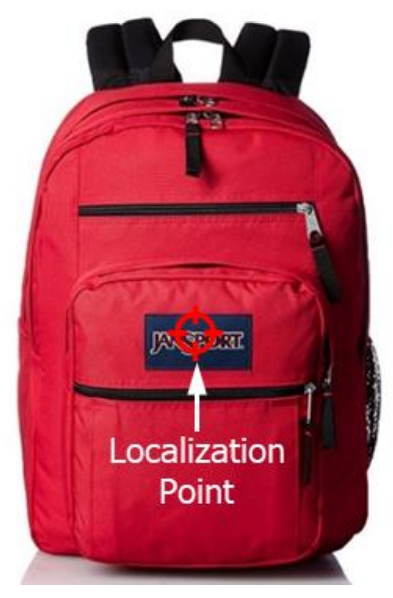
\includegraphics[width=\textwidth]{backpack_artifact.png}
		\caption{Backpack Artifact}
		\label{backpack}		
	\end{subfigure}
	\hfill
	\begin{subfigure}{0.3\textwidth}
		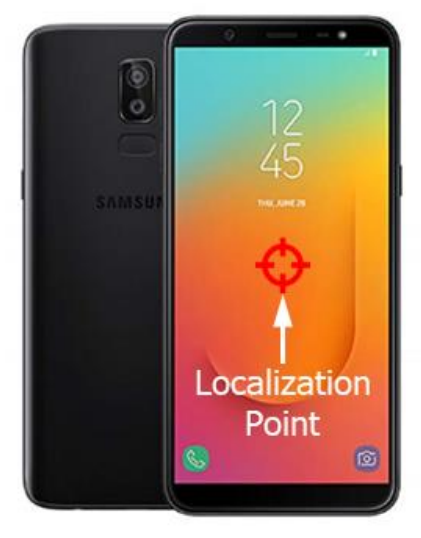
\includegraphics[width=\textwidth]{cell_phone_artifact.png}
		\caption{Cell Phone Artifact}
		\label{cell phone}
	\end{subfigure}	
	\hfill
	\begin{subfigure}{0.3\textwidth}
		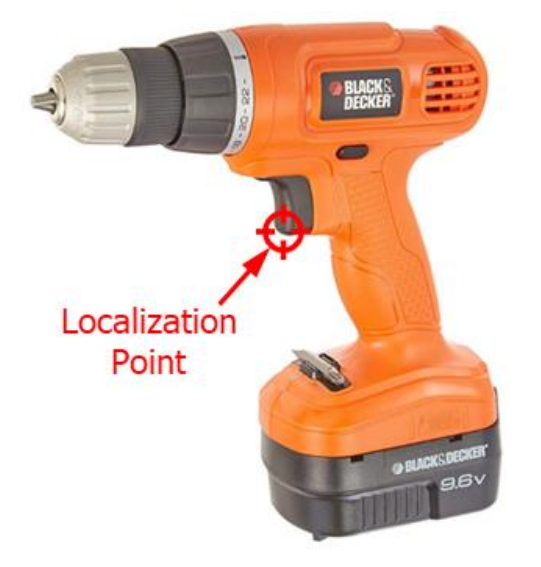
\includegraphics[width=\textwidth]{drill_artifact.png}
		\caption{Drill Artifact}
		\label{drill}
	\end{subfigure}
	\\
	\begin{subfigure}{0.45\textwidth}
		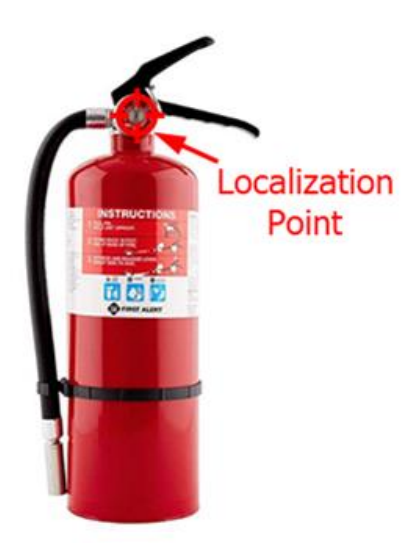
\includegraphics[width=\textwidth]{fire_extinguisher_artifact.png}
		\caption{Fire Extinguisher Artifact}
		\label{fire extinguisher}
	\end{subfigure}	
	\hfill
	\begin{subfigure}{0.45\textwidth}
		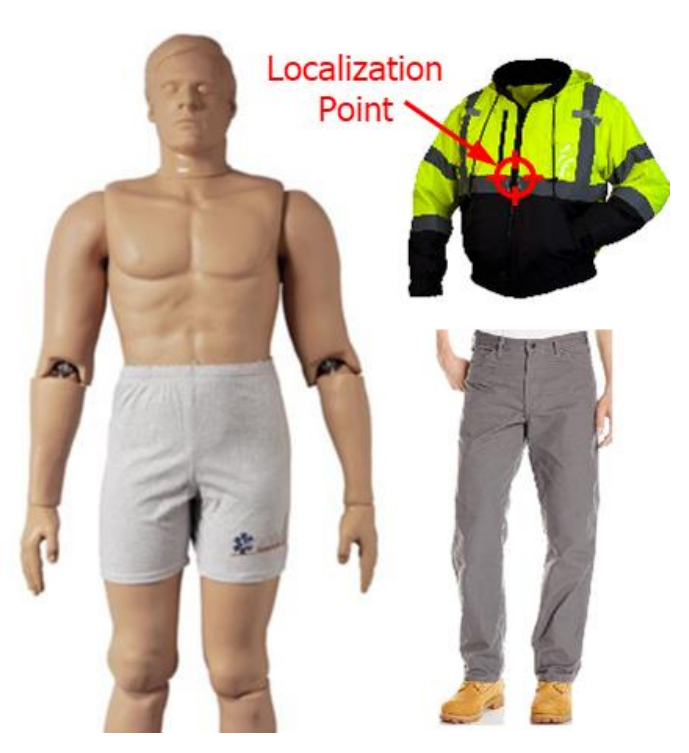
\includegraphics[width=\textwidth]{randy_artifact.png}
		\caption{Survivor Artifact ("Randy")}
		\label{randy}
	\end{subfigure}	
	\caption{Tunnel circuit artifacts}
	\label{tunnel artifacts}
\end{figure}

\section{Related Work}
\chapter{Hardware Development}

One of the cornerstones of our team's Concept of Operations for the SubT Challenge was modular autonomy. That is, we wanted to develop a series of modules which could be composed and rapidly reconfigured to suit the task at hand. The use of individual modules would also allow for components to be replaced or upgraded as necessary. For example, each of our ground robots had 4 drive modules, each consisting of a wheel, motor, gearbox, and a separate electronics module. The drive modules could be replaced or upgraded as necessary, such as in the case of a gearbox failing or the selection of different desired torque profiles. Similarly, we wanted to develop modular sensing and compute payloads which could be transferred across different robots, including in between ground and aerial robots, and which would be capable of performing all of the robot's high level autonomy functions.

Early indication that our approach should be feasible came as the result of using a prototype state estimation payload ("Blue Payload") similar to the Kaarta Traak \cite{kaarta_traak}. The payload was relatively small, self-contained, and could be easily transferred between robots (see Figure \ref{blue payload robots}). We simply had to mount the payload to the robot, apply power, and connect to the robot's internal network, and all of the payload's autonomy functions would be enabled. Overall, we found the Blue Payload quite simple to integrate, and wanted our future payloads to be similar in this regard. Inspired by the Blue Payload, and keeping the SubT Challenge requirements and timeline in mind, we came up with a list of some design goals and desired capabilities for our first payload ("Mk 0"), sorted by priority:

\begin{description}
	\item[Self-contained] All of the sensing and computation for the high level autonomy features should happen inside the payload itself. Ideally, the payload would only be supplied power and a network connection, just like the Blue Payload, and would output autonomy goals (such as waypoints) and information (such as robot state, maps, and artifact locations) to be relayed to the human supervisor at the base station.
	\item[Rapid Development] From the beginning of the competition (September 2018) to the first qualification deadline (December 2018), we had a little under 3 months to develop our first payload. This meant that, wherever possible, we should prefer designs that relied on existing expertise, such as the use of familiar components and sensors, and preferring in-house manufacturing capabilities with short lead times.
	\item[Environmentally Robust] We expected the field environments for the SubT competition to be somewhat hostile to the sensors. Specifically, we were told that "dust, fog, mist, water, and smoke are within scope" \cite{tunnel_rules}, and we wanted our payload to be reasonably protected against these elements, within reason. Additionally, the payload needed to be robust to the mechanical loading it would be subject to as a result of the rough terrain.
	\item[Weight Sensitivity] Similar to the Blue Payload, we wanted our new payload to be light enough to be carried by one of our aerial robots (as in Figure \ref{d1 blue payload}), or a smaller ground robot (as in Figure \ref{joeybot blue payload}) in addition to larger robots (as in Figure \ref{r1 blue payload}).
	\item[Low Cost] While there aren't specific restrictions on the maximum cost of our robot, DARPA was interested in identifying cost effective solutions for the SubT Challenge. Minimizing cost is also useful as a design goal as we intended to build multiple copies of the payload for our various robots, as well as to have spares.
\end{description}

\begin{figure}
	\centering
	\begin{subfigure}{0.3\textwidth}
		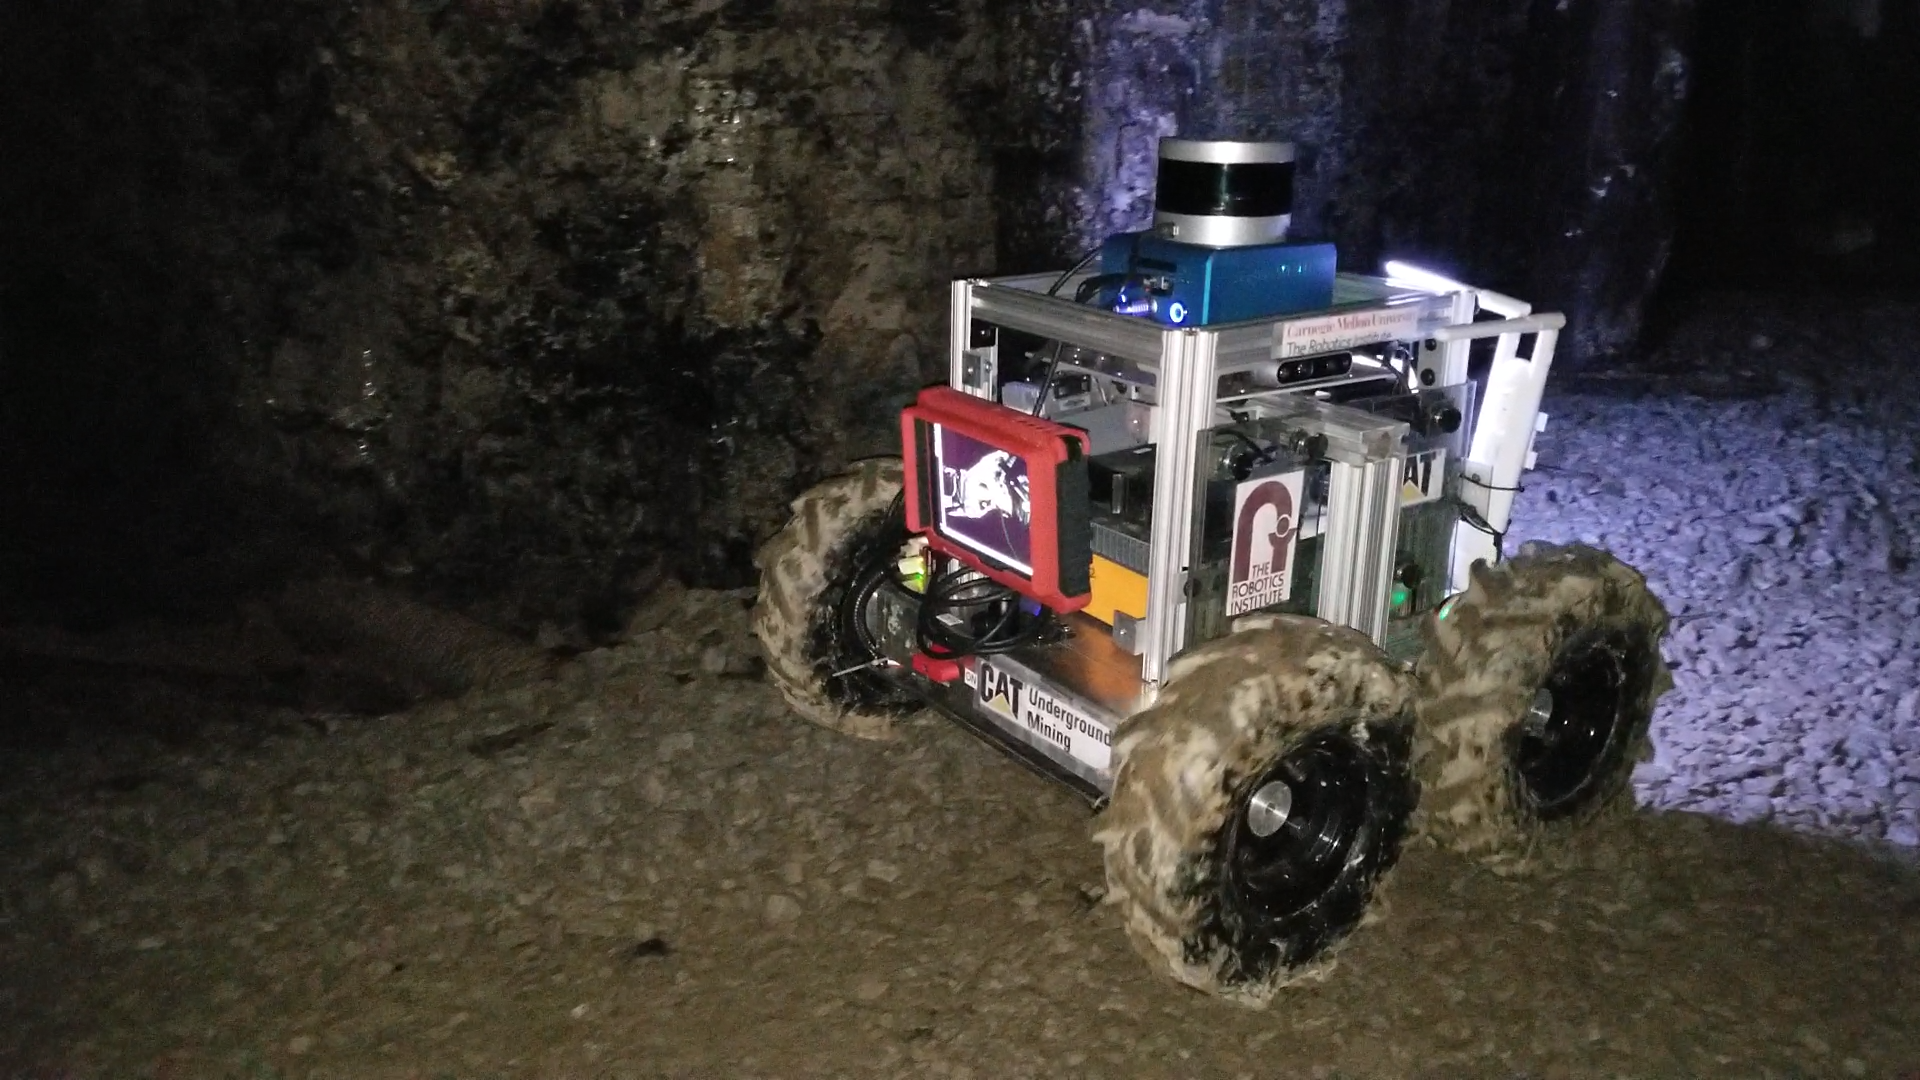
\includegraphics[width=\textwidth]{blue_payload_joeybot.png}
		\caption{Joeybot with Blue Payload}
		\label{joeybot blue payload}
	\end{subfigure}		
	\hfill
	\begin{subfigure}{0.3\textwidth}
		\includegraphics[width=\textwidth]{r1_with_blue_payload.jpg}
		\caption{R1 with Blue Payload}
		\label{r1 blue payload}		
	\end{subfigure}
	\hfill
	\begin{subfigure}{0.3\textwidth}
		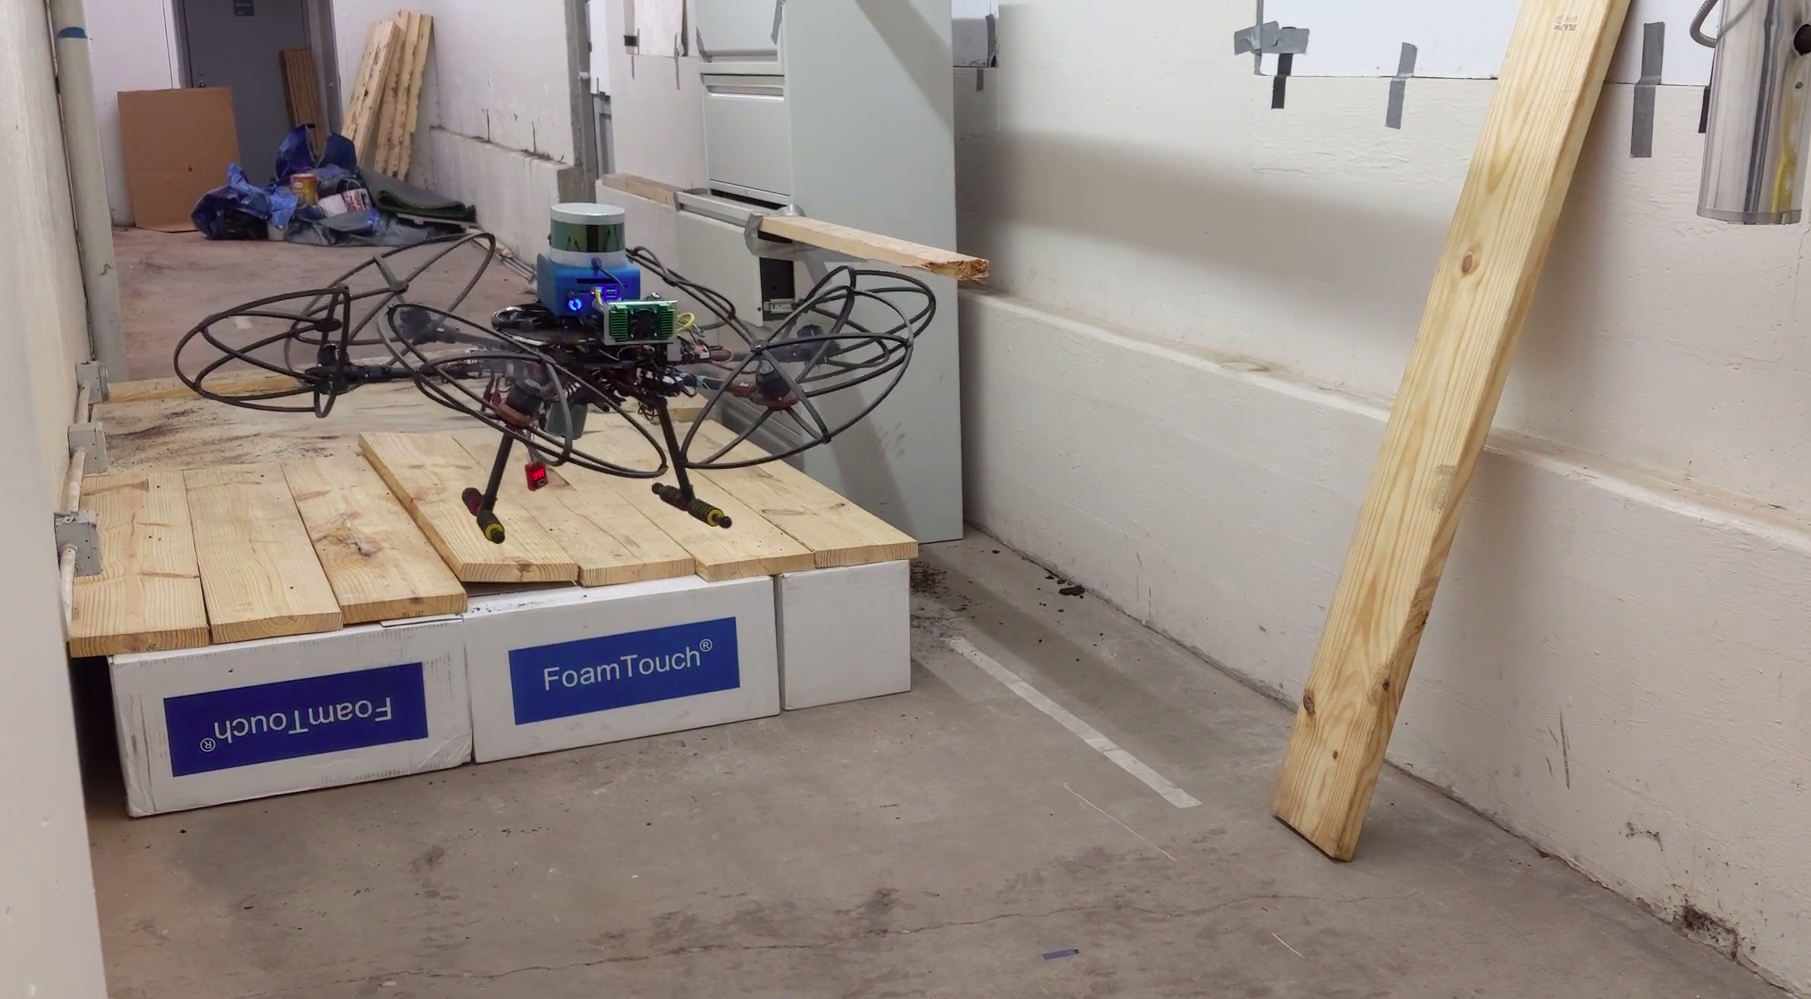
\includegraphics[width=\textwidth]{drone_with_blue_payload.png}
		\caption{D1 with Blue Payload}
		\label{d1 blue payload}
	\end{subfigure}	
	\caption{Robots with initial modular payload ("Blue Payload")}
	\label{blue payload robots}
\end{figure}

\section{Mk. 0 Component Selection}

\subsection{Computers}

In order to select the computer(s) to be used inside Mk. 0, it was important for us to figure out the tasks that the payload would need to perform. While we wouldn't be able to know exactly how many resources each of the tasks would consume, prior experience could help us determine some rough approximations. The main tasks for the payload would be the following:

\begin{enumerate}
	\item State estimation
	\item Path planning and navigation
	\item Object detection and localization
\end{enumerate}

For state estimation, we knew that we would be using LOAM \cite{zhang2014loam}, which was written by Ji Zhang (one of our team members), and is the current state of the art for SLAM. We knew that LOAM ran well on the Blue Payload, which uses an Intel NUC with an Intel Core i7 processor internally. The path planning and navigation stack was being actively developed and ran on the second computer on Joeybot (see Figure \ref{joeybot blue payload}), which was a mid-range industrial-grade PC from Logic Supply. Though the Logic Supply computer was also using an Intel Core i7 processor, the processor itself was underclocked to reduce heat output. Profiling indicated that it should be possible to run the path planning and navigation stack on the NUC being used to run LOAM, especially given the underclocked processor in the Logic Supply computer. This factor, along with various team members' familiarity with the NUC family of products, marked the Intel NUC as a strong contender for use in our payload. Specifically, we considered the NUC8i7BEB, which the best (with regards to CPU) available NUC board at the time.

Working under the assumption that we'd use an Intel NUC inside the payload, the question of running the object detection and localization stack still remained. While it wasn't yet clear what our object detection strategy would be, the use of convolutional neural networks in advancing the state of the art for object detection suggested that they would be a component of our approach. To efficiently run convolutional neural networks, a few hardware platforms were considered. We attempted to find a platform which we thought could run multiple neural networks in parallel, at relatively high frequencies (10+ Hz). We considered the following options:

\begin{enumerate}
	\item Intel Movidius Neural Compute Stick
	\item NUC8i7BEB integrated GPU (Intel Iris Plus Graphics 655)
	\item Nvidia Jetson TX2
	\item Nvidia Jetson AGX Xavier
\end{enumerate}

Of the available options, the Nvidia Jetson AGX Xavier ("Xavier") offered the highest inference performance due to its many CUDA cores, as well as its specialized Tensor Cores and Deep Learning Accelerators. Combined, the Xavier was capable of performing more than an order of magnitude more FLOPS than the other platforms. As we were unsure of the exact requirements of our object detection system at the time, we chose to overprovision, and thus the available FLOPS became the deciding factor. The Xavier emerged as the clear winner for our GPU selection inside the Mk. 0 payload. At this stage, it was also decided to commit to using the NUC8i7BEB inside Mk. 0. In an attempt to simplify the system, we briefly considered attempting to run the entire autonomy stack on a single Xavier, rather than split between a NUC and an Xavier. However, we felt that the slower ARM cores on the Xavier would not be able to handle the combined autonomy stack, and thus decided to continue using both computers inside the Mk. 0 payload. The NUC would handle the state estimation and path planning and navigation tasks while all object detection and localization tasks would run on the Xavier.

After the completion of the Mk. 0 payload, we performed some experiments to see if our earlier hypothesis about the Xavier being unable to handle the entire autonomy stack was correct. Profiling of the NUC revealed that LOAM was one of the heaviest processes, consuming nearly 100\% of a single core in some circumstances, and smaller portions of other cores. Thus, we decided to attempt to run LOAM on the Xavier first. For our benchmarking, we set up an Xavier Developer Kit in MAX-N mode after having disabled the frequency governors with the provided jetson\_clocks.sh script. This mode enables all of the processors in the Xavier, and pins them at their highest frequency. We attempted to run LOAM on pre-recorded data in a few different configurations, varying a parameter to adjust downsampling of the input point clouds to reduce the scan alignment cost. Figure \ref{loam_xavier} shows a visualization of the results.

\begin{figure}
	\centering
	\begin{subfigure}{0.3\textwidth}
		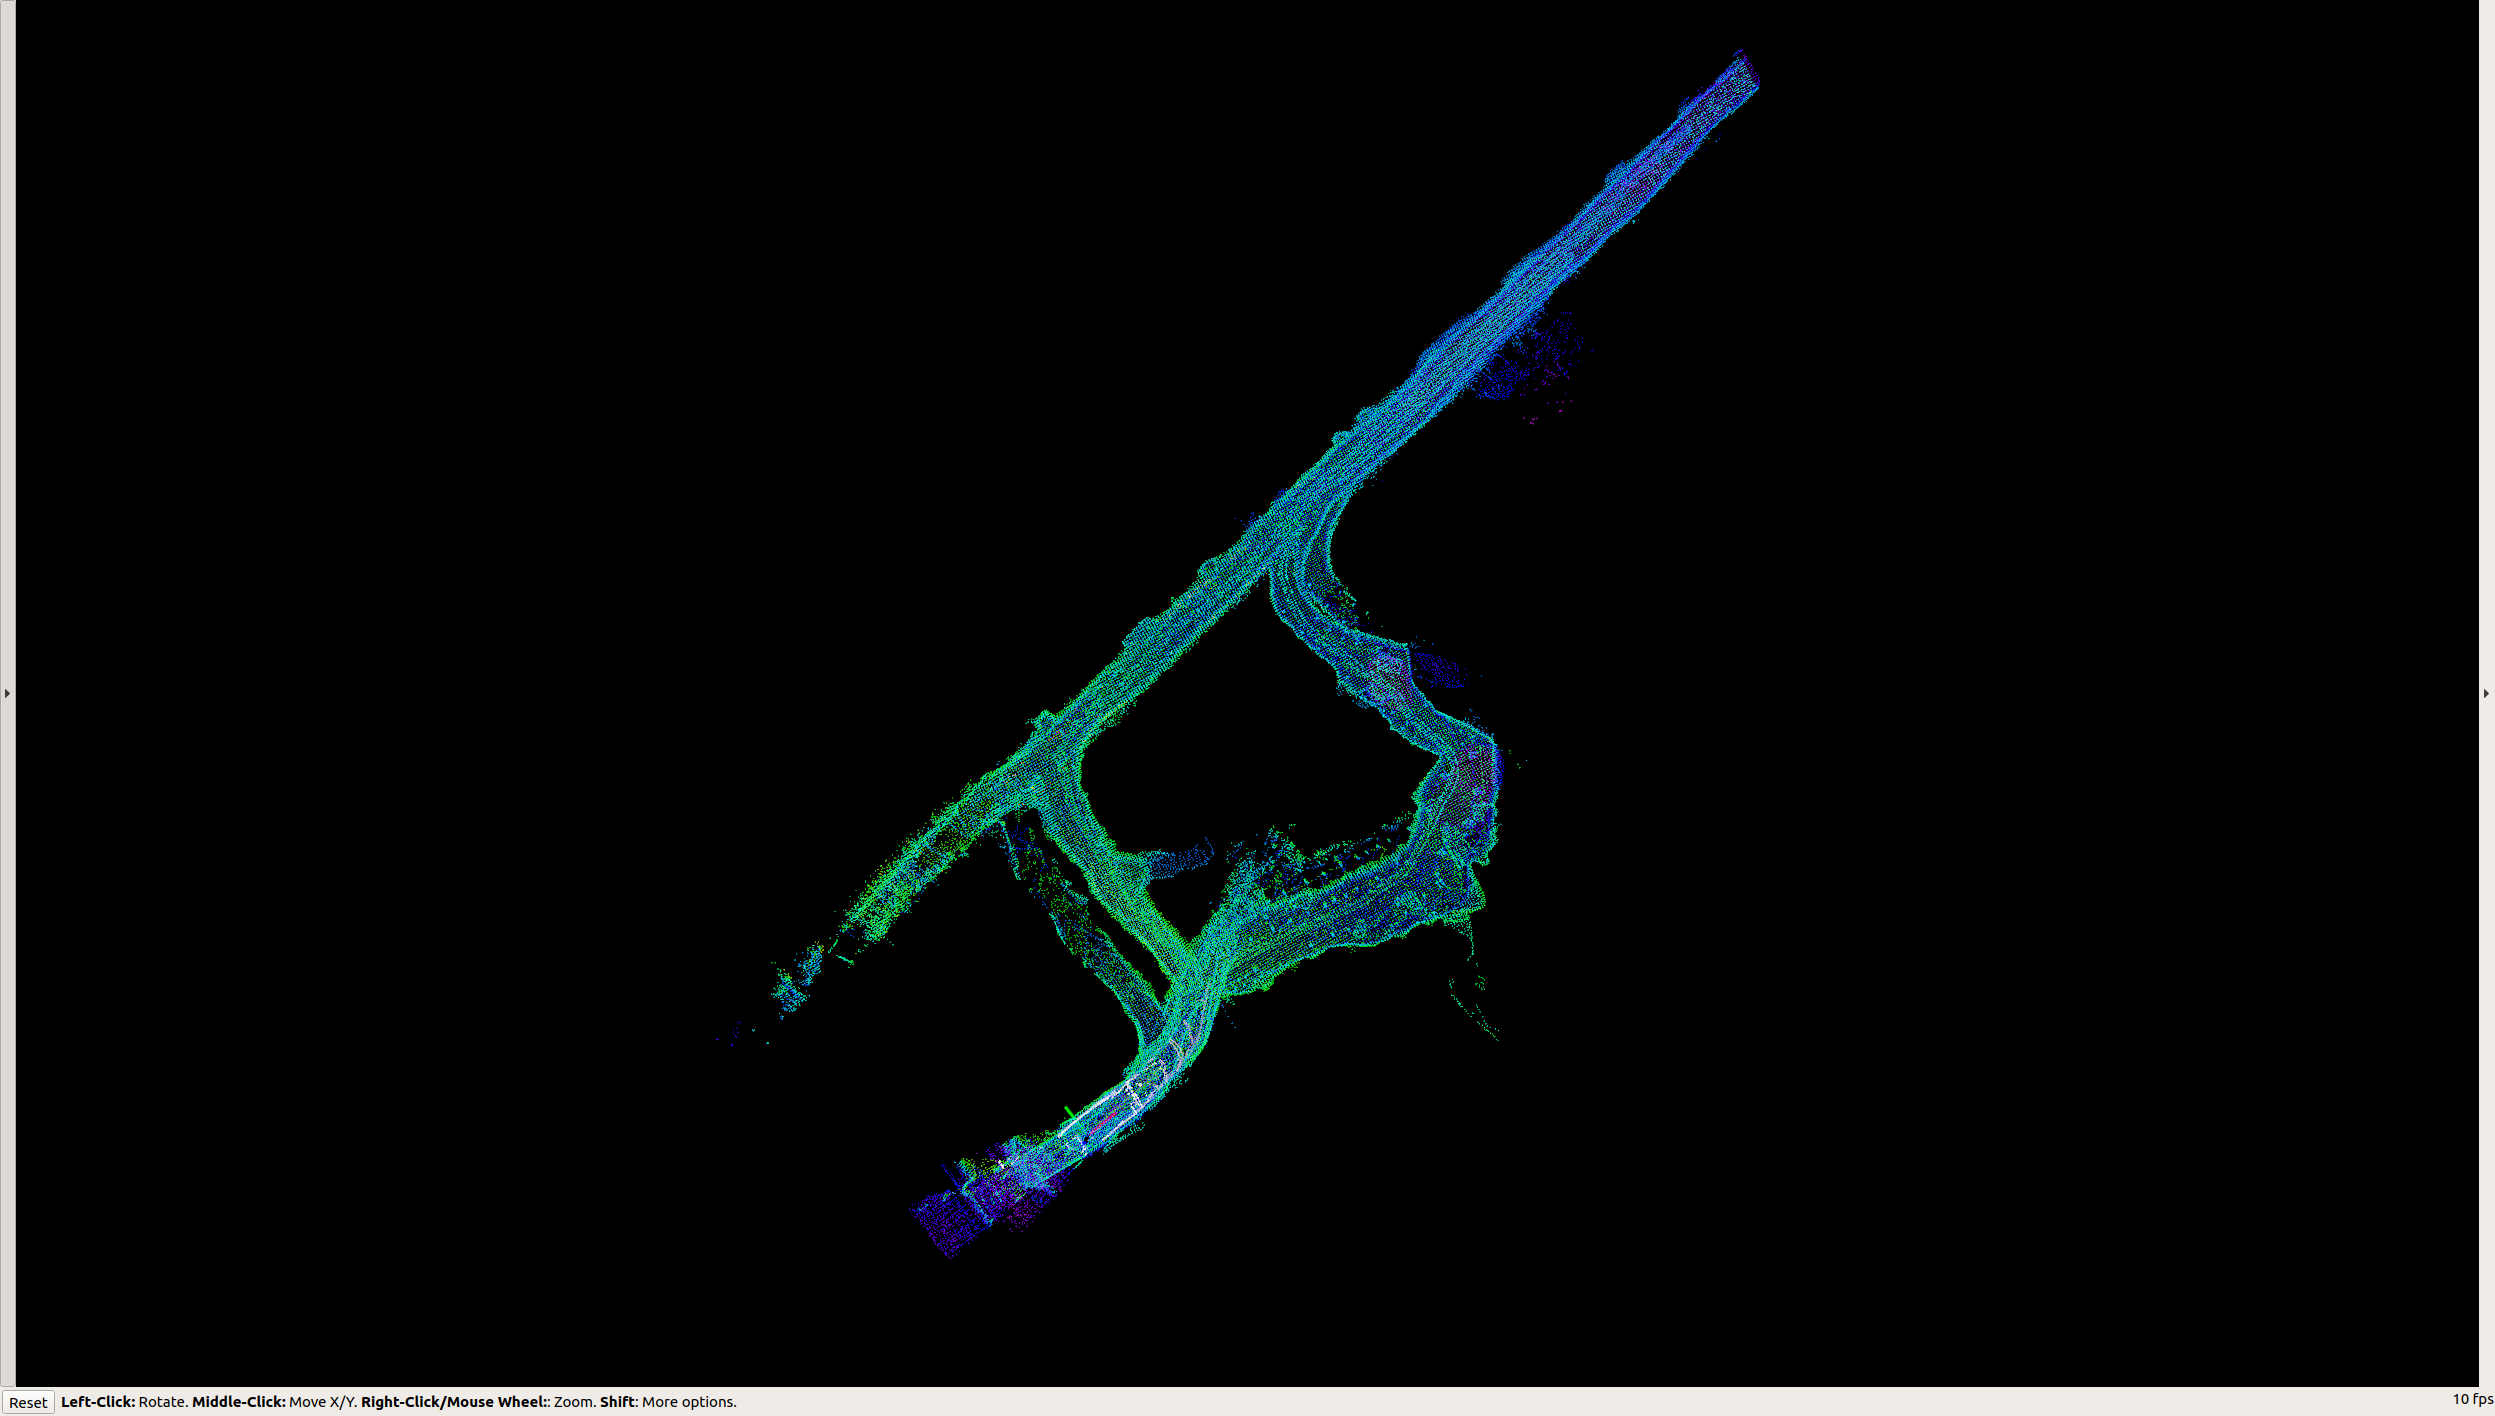
\includegraphics[width=\textwidth]{tour_ed_mine_1-00.png}
		\caption{100\% Point Cloud Scaling}
		\label{loam_xavier_100}
	\end{subfigure}		
	\hfill
	\begin{subfigure}{0.3\textwidth}
		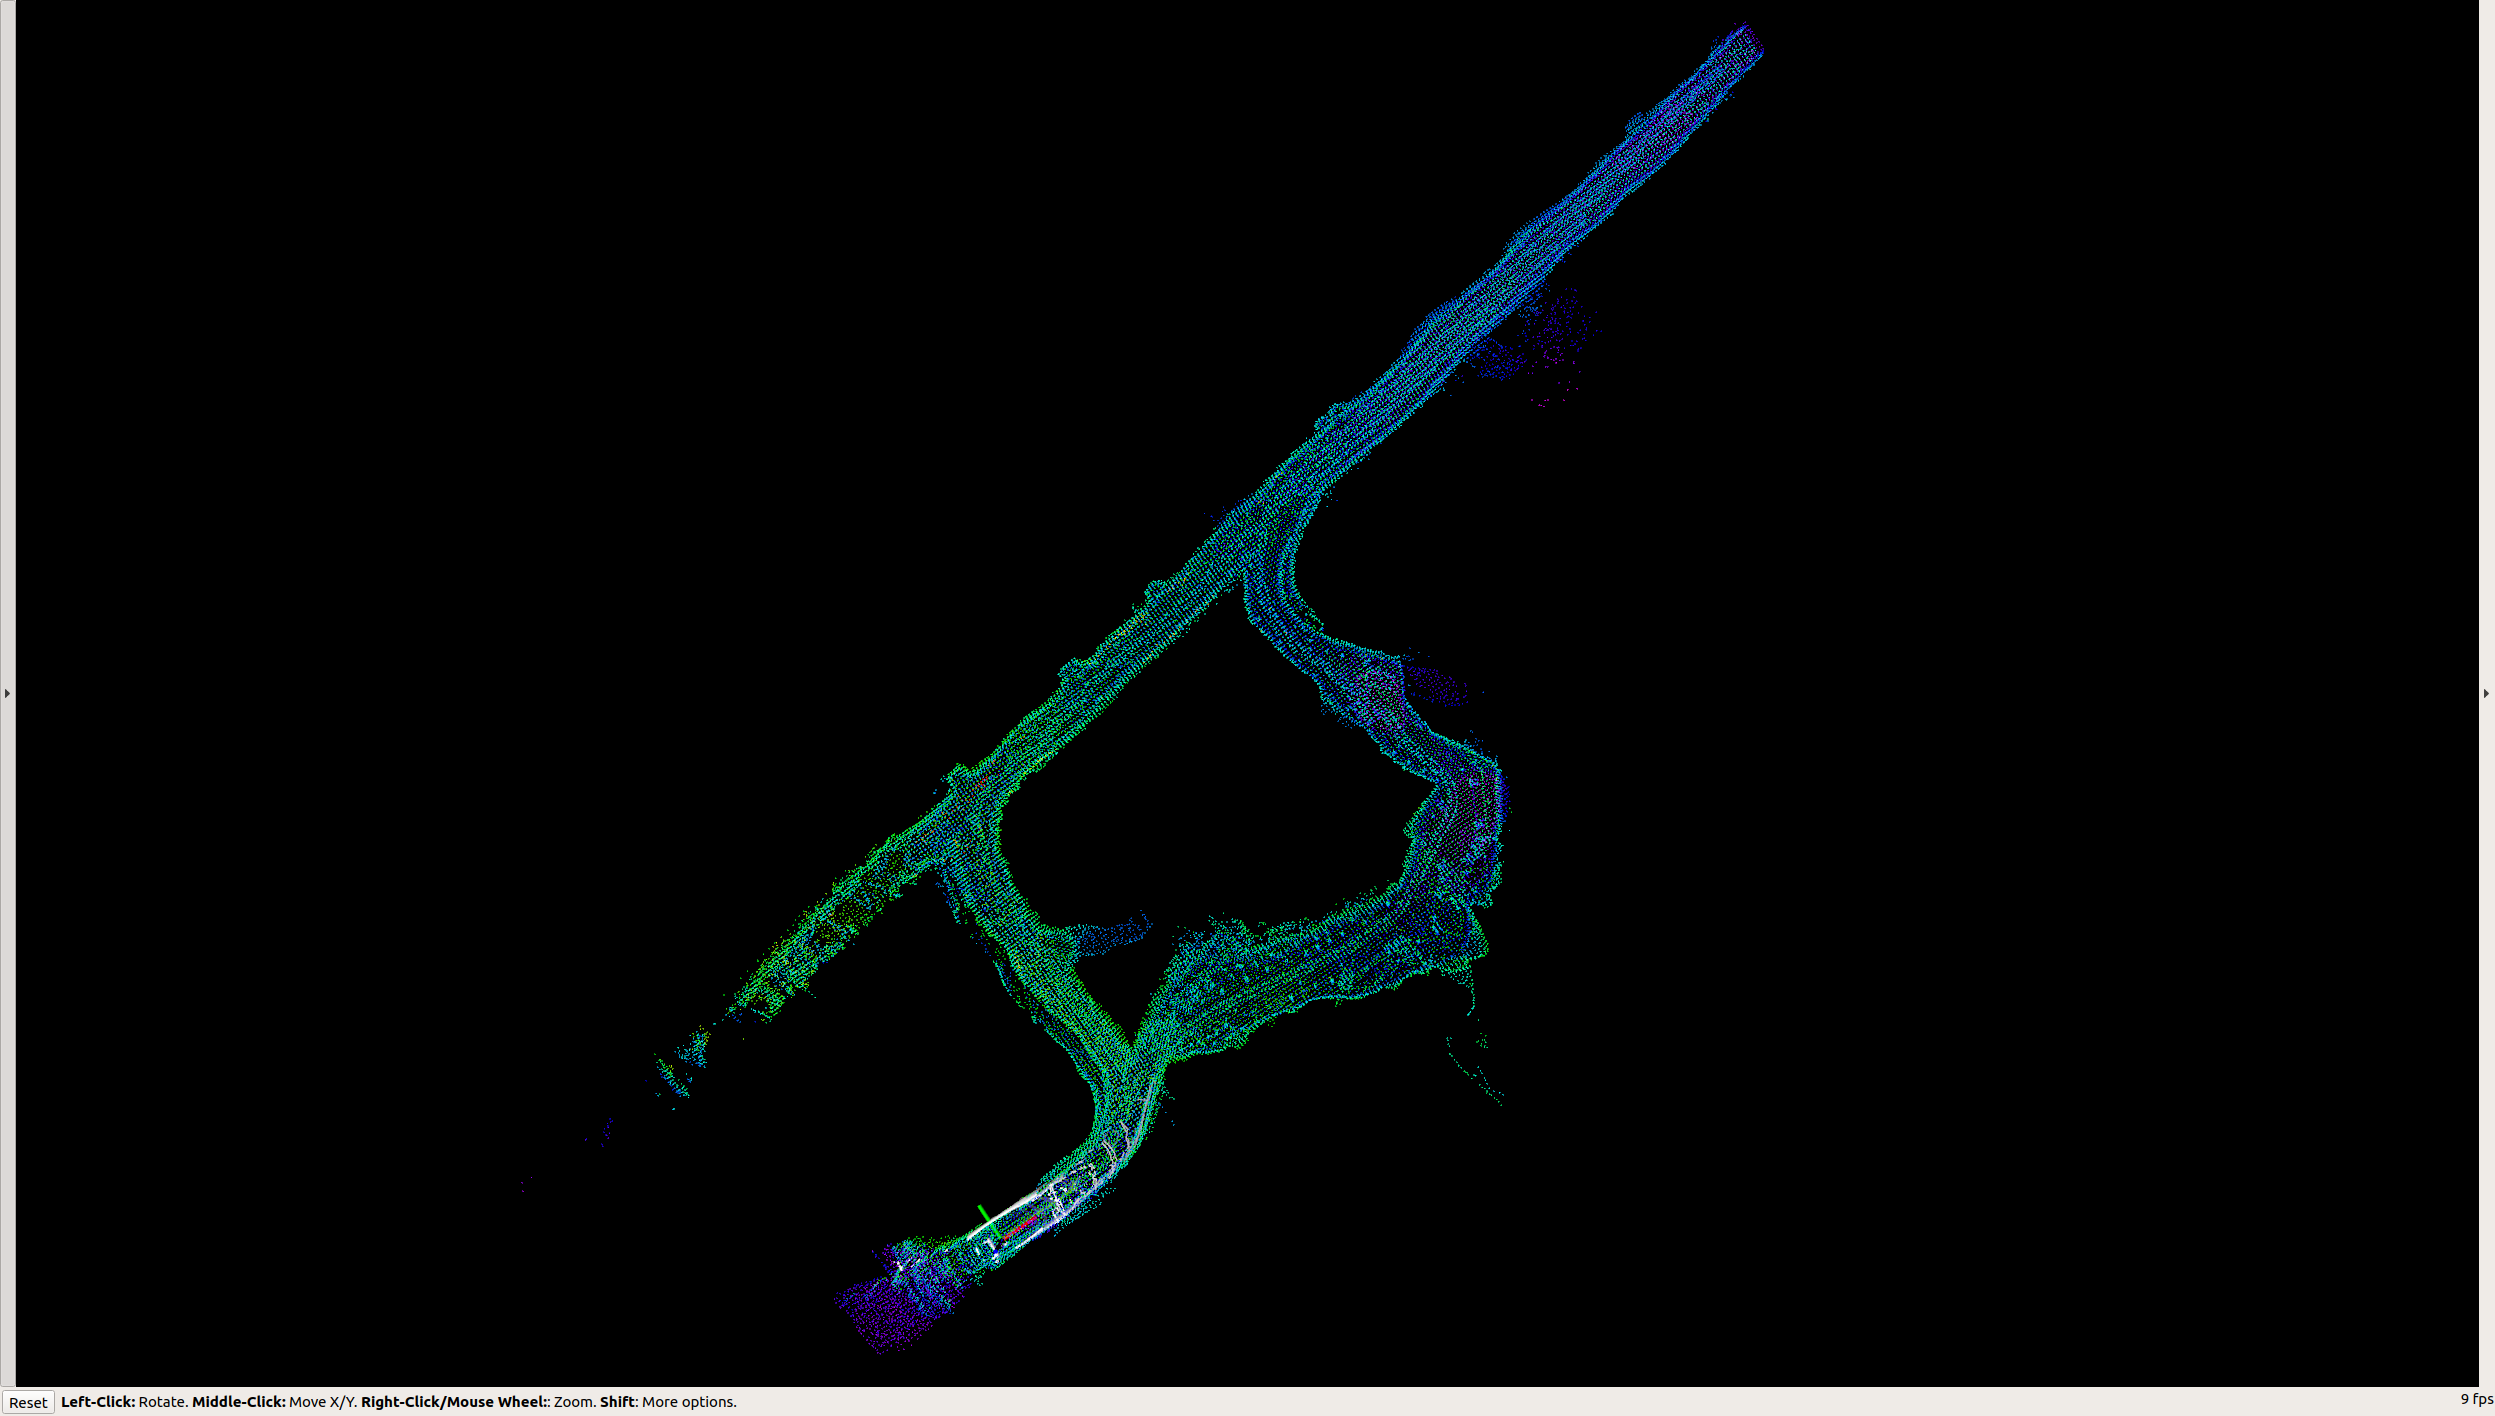
\includegraphics[width=\textwidth]{tour_ed_mine_1-00_1-25s.png}
		\caption{75\% Point Cloud Scaling}
		\label{loam_xavier_75}		
	\end{subfigure}
	\hfill
	\begin{subfigure}{0.3\textwidth}
		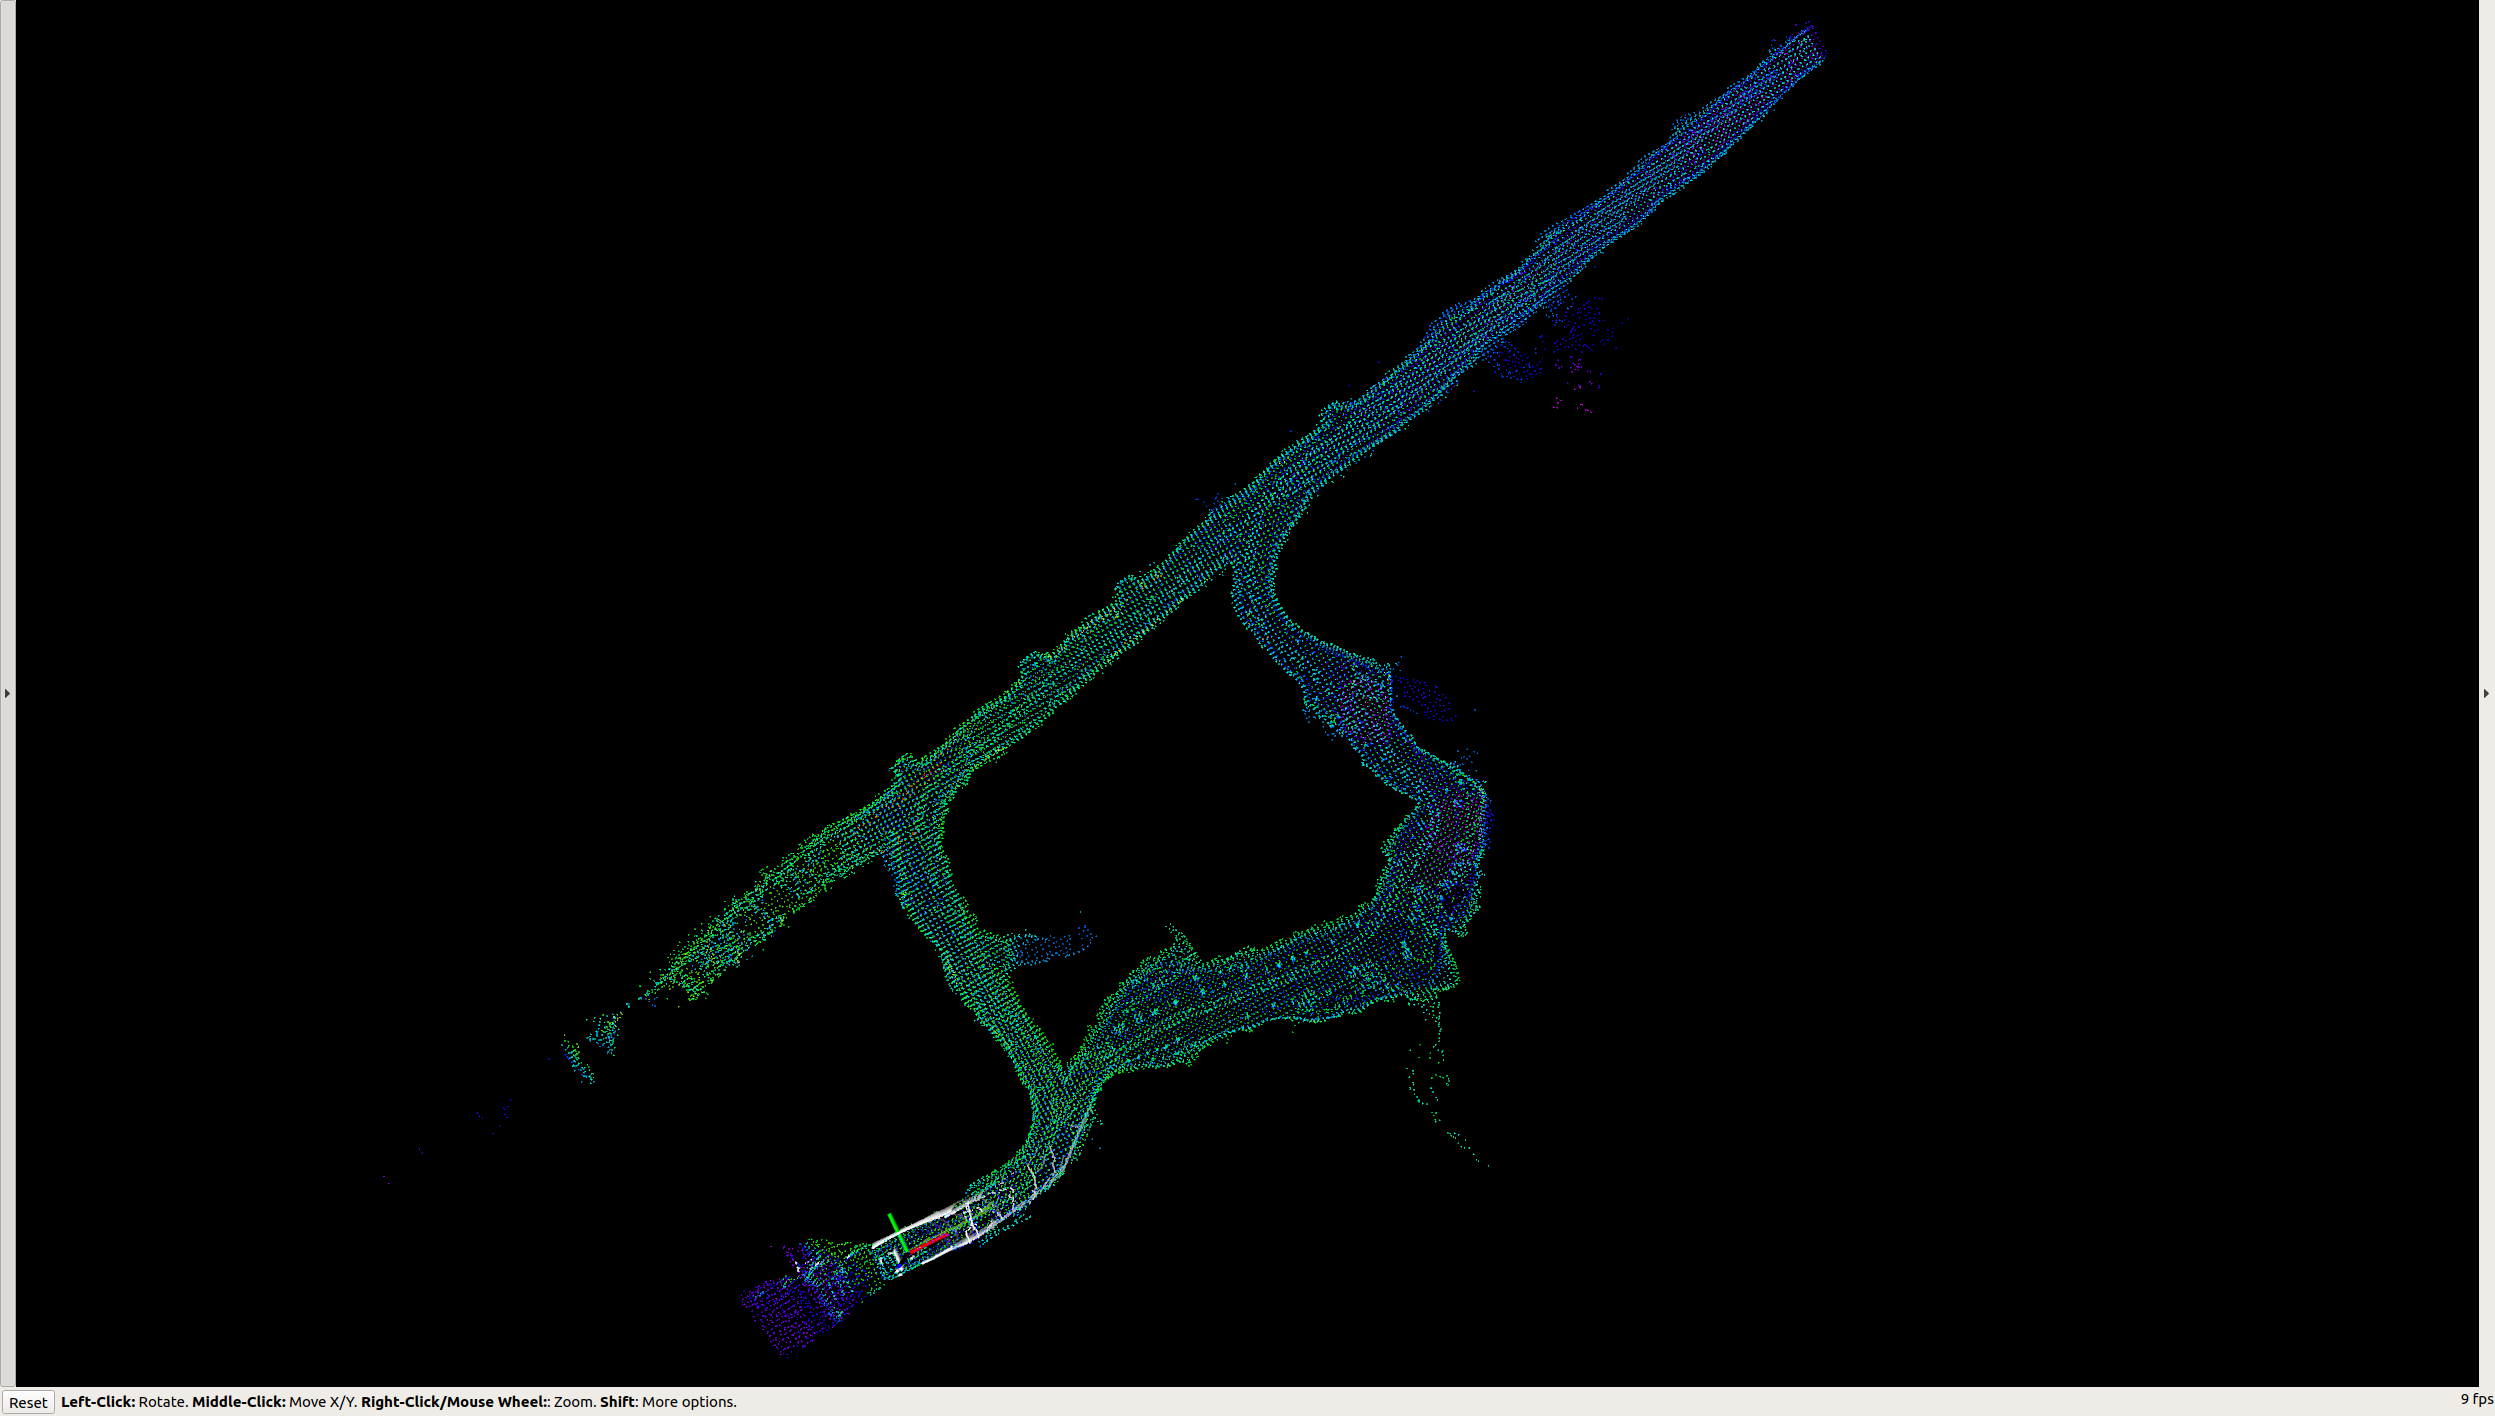
\includegraphics[width=\textwidth]{tour_ed_mine_1-00_1-50s.png}
		\caption{50\% Point Cloud Scaling}
		\label{loam_xavier_50}
	\end{subfigure}	
	\caption[Visualization of LOAM running on an Xavier]{Visualization of LOAM running on an Xavier with different downsampling parameters, using pre-recorded data collected at the Tour-Ed Mine in Tarentum, PA.}
	\label{loam_xavier}
\end{figure}

In Figure \ref{loam_xavier_100}, the same configuration as the NUC on Mk. 0 was used. Severe misalignment is visible - the lower tunnel does not align correctly, and a secondary "ghost" tunnel is created. In Figure \ref{loam_xavier_75}, 75\% of the laser scanner's points are kept. This does result in better alignment, though the images of two tunnels are still clearly visible in the figure. Finally, in Figure \ref{loam_xavier_50}, only 50\% of the laser scanner's points are kept. In this environment, the point cloud alignment is successful, suggesting that the state estimate did not drift significantly. However, the requisite 50\% downsampling was deemed to be too significant, as it presented a high risk of misalignment under harsh motions or in feature-bare environments due to the low density of points. This experiment confirmed our initial hypothesis that, without significant optimization, our current autonomy stack would be unable to run on a single Xavier.

\subsection{Sensors}

The first set of sensors selected for Mk. 0 were those necessary for state estimation. We selected exactly the same IMU and LIDAR (Velodyne VLP-16 Puck) as were used on the Blue Payload since LOAM was already proven to work with them. We then attempted to determine which sensors we would need to be able to identify all of the artifacts in the challenge. At this point in the competition, DARPA had not released a specific list of artifacts that would be used in the challenge, only general categories \cite{tunnel_rules}. We created a list of the types of sensors which we felt we could integrate into Mk. 0 in the short time available, and estimated the usefulness of each category of sensor in detecting artifacts from each category. A summary is presented in Table \ref{sensor_utility_categories}. The values were decided as follows:

\begin{itemize}
	\item High -- Artifacts of this category are expected to produce extreme sensor responses and be easy to distinguish.
	\item Medium -- Artifacts of this category are expected to be found with moderate difficulty in sensor data.
	\item Low -- Artifacts of this category are expected to be difficult or expensive to separate from sensor noise, perhaps due to a low response, or anticipated interference.
	\item None -- Artifacts of this category are expected to effect no response in sensors of this category.
\end{itemize}

% TODO(vasua): Do I need to add more information about how I came up with this table?

% https://www.tablesgenerator.com/#
\begin{table}[]
	\centering
	\resizebox{\textwidth}{!}{%
		\begin{tabular}{lccccccc}
			\hline
			& \textbf{\begin{tabular}[c]{@{}c@{}}RGB\\ Camera\end{tabular}} & \textbf{\begin{tabular}[c]{@{}c@{}}Thermal\\ Camera\end{tabular}} & \textbf{\begin{tabular}[c]{@{}c@{}}Depth\\ Camera\end{tabular}} & \textbf{LIDAR} & \textbf{Microphone(s)} & \textbf{\begin{tabular}[c]{@{}c@{}}Wifi / Bluetooth\\ Scanning\end{tabular}} & \multicolumn{1}{l}{\textbf{Gas Sensor}} \\ \hline
			\textbf{Survivors}                  & High                                                          & High                                                              & High                                                            & Medium         & Low                    & None                                                                         & None                                    \\ \hline
			\textbf{Ingress / Egress Points}    & Medium                                                        & Low                                                               & High                                                            & Medium         & Low                    & None                                                                         & Low                                     \\ \hline
			\textbf{Electric Pumps}             & High                                                          & High                                                              & Low                                                             & Medium         & Medium                 & None                                                                         & None                                    \\ \hline
			\textbf{Backpacks}                  & High                                                          & None                                                              & Low                                                             & Low            & None                   & None                                                                         & None                                    \\ \hline
			\textbf{Valves}                     & High                                                          & None                                                              & Low                                                             & None           & None                   & None                                                                         & None                                    \\ \hline
			\textbf{Radios / Cell Phones}       & Low                                                           & Medium                                                            & Low                                                             & None           & Medium                 & High                                                                         & None                                    \\ \hline
			\textbf{Tools / Fire Extinguishers} & High                                                          & None                                                              & Low                                                             & None           & None                   & None                                                                         & None                                    \\ \hline
			\textbf{Power Sources}              & Medium                                                        & High                                                              & Medium                                                          & Medium         & None                   & None                                                                         & None                                    \\ \hline
			\textbf{Oxygen Level}               & None                                                          & None                                                              & None                                                            & None           & None                   & None                                                                         & High                                    \\ \hline
			\textbf{Gas Leaks}                  & None                                                          & Medium                                                            & None                                                            & None           & Medium                 & None                                                                         & High                                    \\ \hline
		\end{tabular}%
	}
	\caption{Speculated utility of various sensor categories for DARPA provided artifact categories}
	\label{sensor_utility_categories}
\end{table}

Table \ref{sensor_utility_categories} indicates that while there is some redundancy across sensing categories in their speculated ability to detect various artifact categories, most of the sensor types have at least one artifact category that they alone would be highly likely to detect. For example, Wifi / Bluetooth Scanning is the only sensing category rated as "High" utility in detecting Radios / Cell Phones. Based on this table, Mk. 0 should contain at least some sort of RGB camera, thermal camera, depth camera, wifi / bluetooth scanner, and gas sensor in order to have a high chance of detecting each of the possible artifact categories. A LIDAR isn't required for object detection, but will necessarily be included for state estimation as described above. The microphone isn't strictly necessary, so we aimed to include it in the payload if it would be simple to do, but otherwise devote little attention to it. With our list of sensor types decided, we began experimenting with various products to identify specific models destined for inclusion in Mk. 0.

\begin{description}
	\item[RGB Camera] Having the highest overall utility across sensor categories, the RGB camera was the first sensor we aimed to select. The first selection criteria for the camera was the interface type. Three possibilities were considered -  CSI, Ethernet, and USB. CSI, capable of offering very high data rates with low latency, was the preferred interface. However, hardware and driver support for CSI cameras for the Xavier was still developing at this time, eliminating this option. Ethernet was considered for ease of integration. However, the larger size of Ethernet cameras and connectors, as well as the lower available bandwidth for multiple cameras forced us to eliminate this option as well. We were left with USB as our selection for camera interface. USB 3.0 offered the data rates we would need to use multiple cameras, but had the potential to suffer from high latency due to multiple levels of hardware and software buffering.
	
	With our choice of interface made, we considered two types of cameras for use in the Mk. 0 payload. The first was the UI-3241LE-C-HQ by IDS Imaging, a bare camera board that other members of our lab had successfully used on previous projects. The second was the Intel RealSense D435, selected for its inclusion of a stereo depth pair in a small form factor. When comparing the two cameras, in addition to the overall payload goals, there were a few camera-specific criteria we used when comparing the various cameras:
	
	\begin{enumerate}
		\item Low light performance - We expected the subterranean environments to dimly lit in general, and occasionally be completely dark. A camera with lower image noise in dark environments was preferred.
		\item Synchronization ability - Given the expected utility of the RGB cameras, as well as for redundancy, we anticipated using multiple cameras on Mk. 0. A hardware synchronization mechanism between the cameras and other payload sensors (e.g. LIDAR) would help increase the accuracy of various software algorithms.
		\item Shutter type - A global shutter was preferred due to the increased image quality under harsh camera motions, which was expected as a result of rough terrain.
	\end{enumerate}
	
	% TODO(vasua):  Provide additional images in the appendix, maybe? Not sure how necessary they are.
	To evaluate low light performance, we used the provided ROS drivers to capture images from both cameras at their native / recommended resolutions (1280 x 1024 for the UI camera, and 848 x 480 for the RealSense) across a range of manually selected exposure and gain values with the camera framerates set to 30 fps. The images shown in Figure \ref{camera_comparison} contain images of the same scene from both cameras with 33 ms exposure time and the minimum and maximum gains supported by the drivers. Additionally, images of a similar scene were captured with autoexposure enabled in each camera.
	
	\begin{figure}
		\centering
		\begin{subfigure}{0.3\textwidth}
			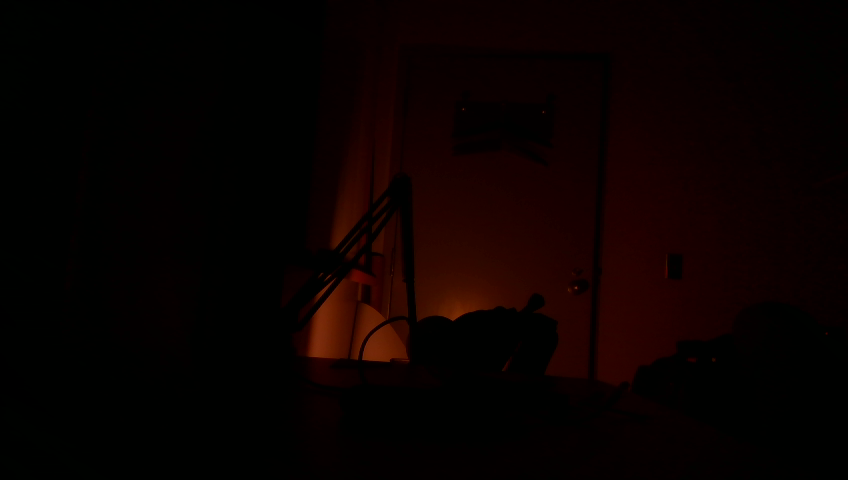
\includegraphics[width=\textwidth]{rs_img_33_ms_016.png}
			\caption{RealSense 33 ms exposure, minimum gain}
			\label{rs_img_33_ms_016}
		\end{subfigure}		
		\hfill
		\begin{subfigure}{0.3\textwidth}
			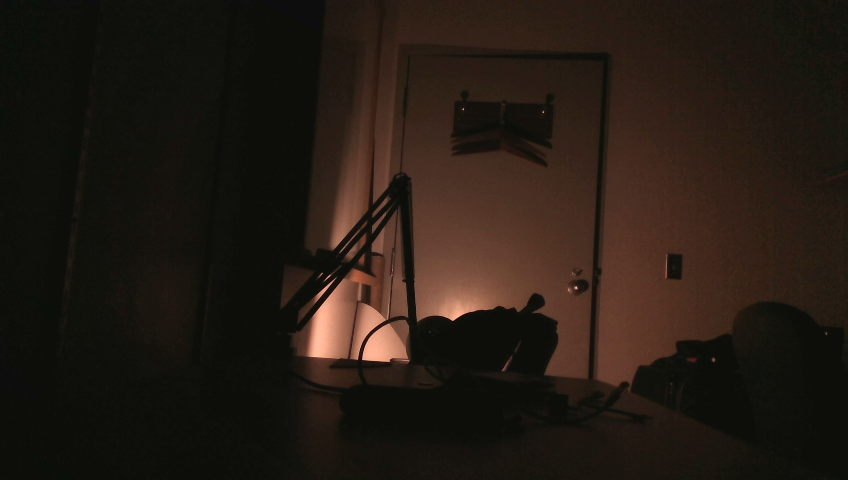
\includegraphics[width=\textwidth]{rs_img_33_ms_128.png}
			\caption{RealSense 33 ms exposure, maximum gain}
			\label{rs_img_33_ms_128}		
		\end{subfigure}
		\hfill
		\begin{subfigure}{0.3\textwidth}
			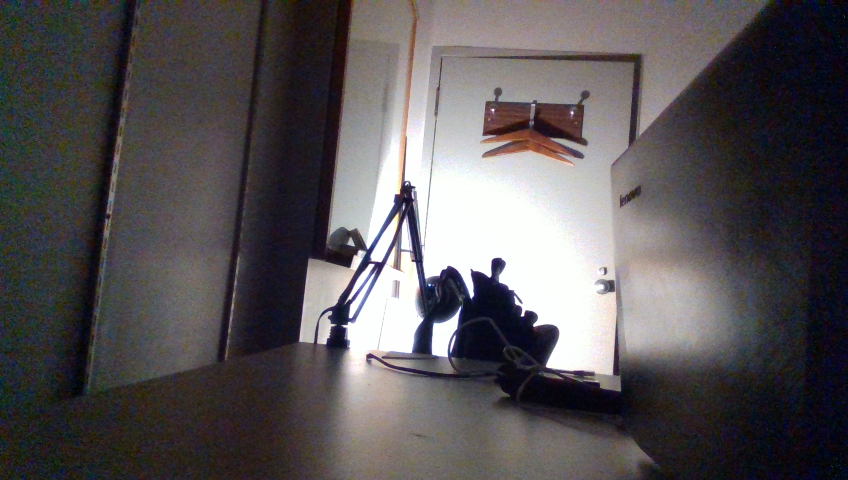
\includegraphics[width=\textwidth]{auto_realsense_2.png}
			\caption{RealSense automatic exposure, automatic gain}
			\label{auto_realsense_2}
		\end{subfigure}
		\\
		\begin{subfigure}{0.3\textwidth}
			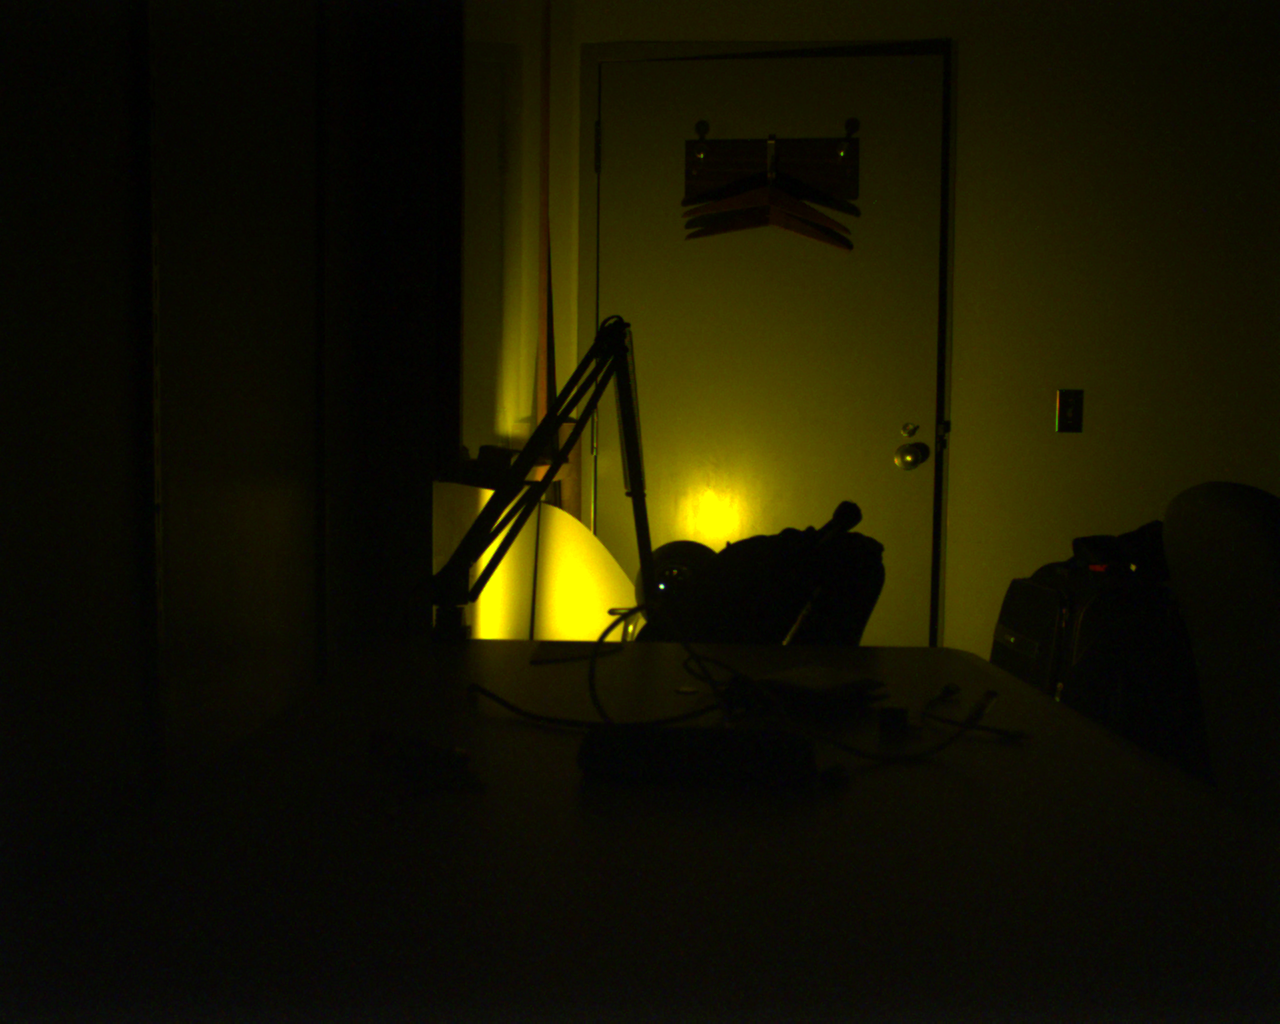
\includegraphics[width=\textwidth]{ui_img_33_ms_000.png}
			\caption{UI 33 ms exposure, minimum gain}
			\label{ui_img_33_ms_000}
		\end{subfigure}		
		\hfill
		\begin{subfigure}{0.3\textwidth}
			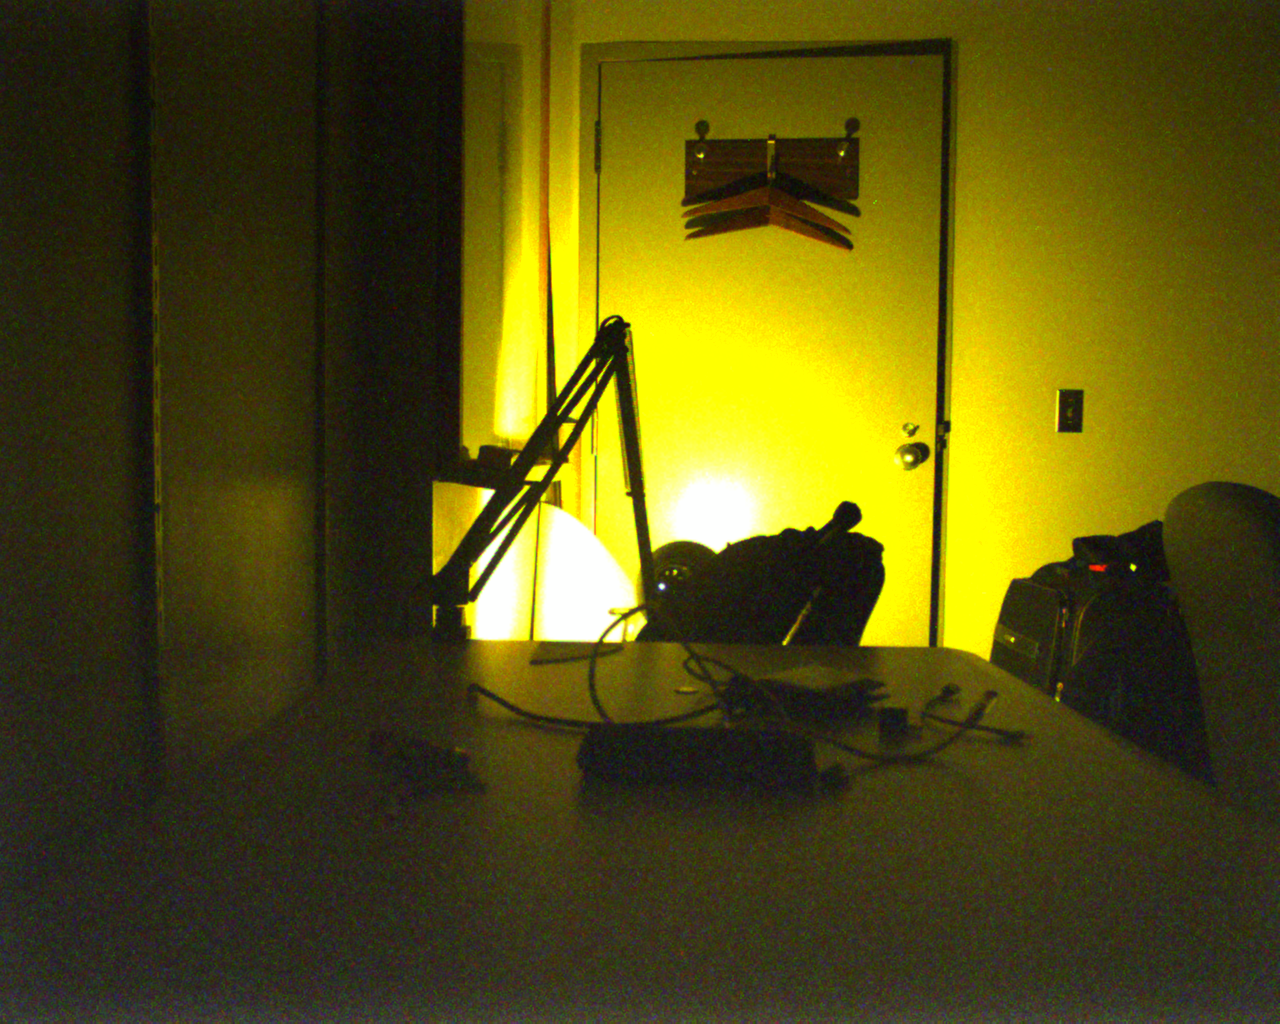
\includegraphics[width=\textwidth]{ui_img_33_ms_100.png}
			\caption{UI 33 ms exposure, maximum gain}
			\label{ui_img_33_ms_100}		
		\end{subfigure}
		\hfill
		\begin{subfigure}{0.3\textwidth}
			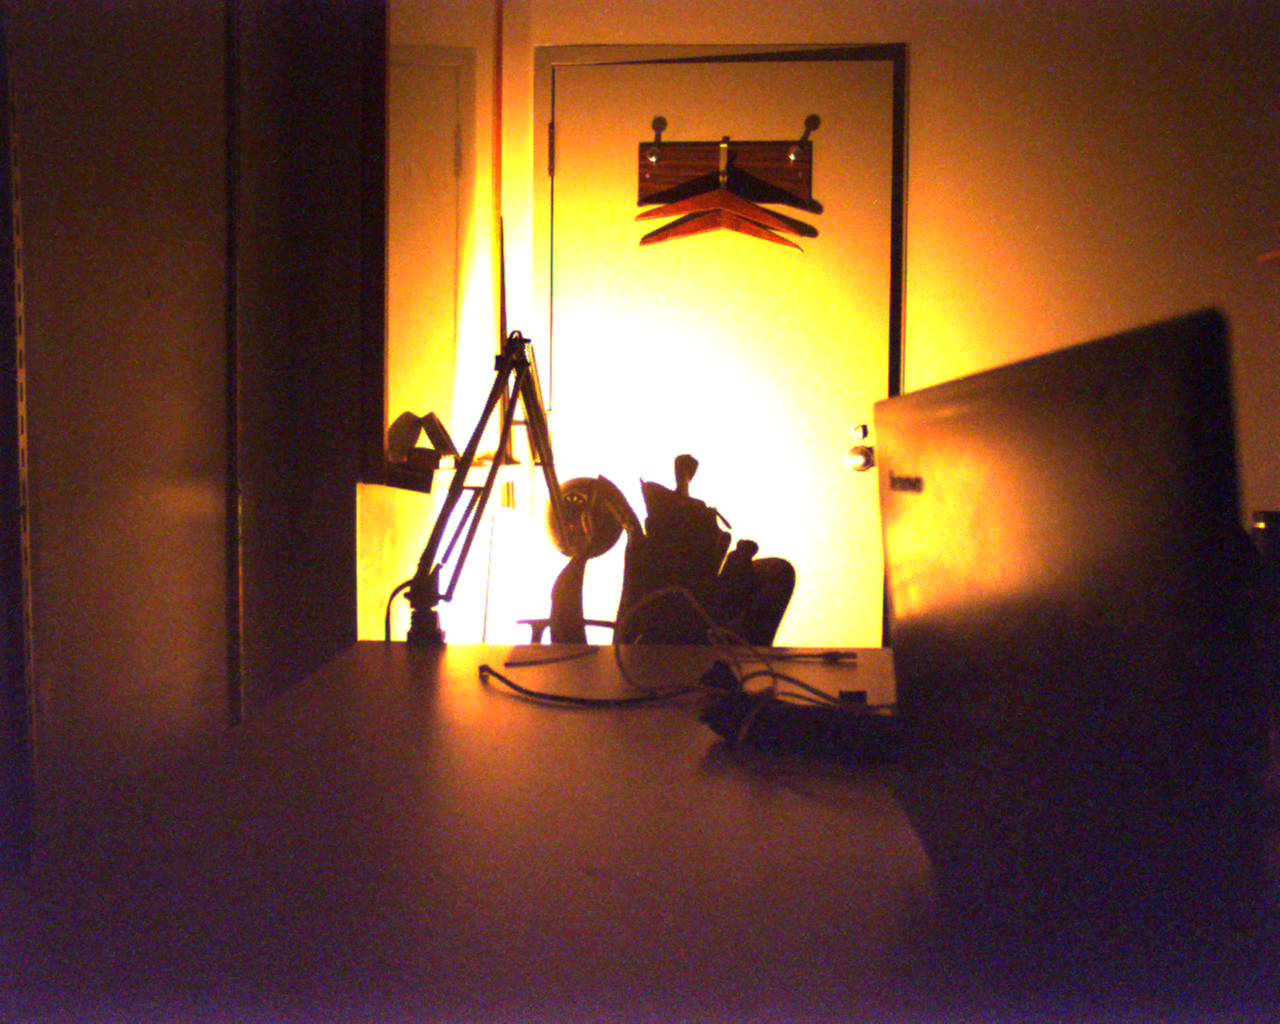
\includegraphics[width=\textwidth]{auto_ueye_2.png}
			\caption{UI automatic exposure, automatic gain}
			\label{auto_ueye_2}
		\end{subfigure}		
		\caption[RGB camera image quality comparison]{Comparison of image quality from UI-3241LE-C-HQ and RealSense D435 RGB cameras across a variety of gain values. Automatic exposure was limited to 33 ms due to a specified framerate of 30 fps for both cameras.}
		\label{camera_comparison}
	\end{figure}

	With manual gain enabled on both cameras, the images from the RealSense RGB camera are less bright, but exhibit significantly less noise than the images from the UI camera. Additionally, the UI camera's image at maximum gain \ref{ui_img_33_ms_100} saturated in the center, while the RealSense image did not, suggesting a lower dynamic range on the UI camera. When autoexposure was enabled on both cameras (\ref{auto_realsense_2}, \ref{auto_ueye_2}), the RealSense exhibited comparable noise to the UI camera, but produced an image with colors more accurate to the actual scene.
	
	When comparing synchronization ability, it appeared at first glance that both cameras supported external frame triggering, which allows frame capture to be driven by an external clock. This feature had previously been validated on the UI cameras in other lab projects. However, upon closer inspection it appeared that the external trigger for the RealSense module only applied to the depth module, and use of the external trigger would remove the synchronization between the RGB and depth modules on the RealSense camera. Similarly, when comparing shutter types, it appeared at first glance that both cameras had global shutters. This has also been previously validated on the UI cameras in other lab projects. However, further investigation revealed that the RealSense had a global shutter only for the 2 IR cameras used to compute depth, with the RGB camera instead having a rolling shutter.
	
	After this experiment, we decided to choose the RealSense D435 module for the Mk. 0 payload. We believed that the increase in low light image quality would outweigh the lack of external triggering and RGB camera rolling shutter. Additionally, the RealSense contained a depth module which eliminated the need for the selection of a separate depth camera. The RealSense also beat the UI camera in other payload goals - its price was less than half that of the UI camera, had shorter lead times which would allow for more rapid development, and had an enclosure which would simplify keeping the payload environmentally robust compared to the bare UI camera board.
	
	% TODO(vasua): Is there a better place for this to go? Maybe a footnote?
	It should be noted that after this experiment was performed, it was discovered that the RealSense firmware version used had a bug when setting manual gain which lowered the maximum possible gain value. The automatic gain feature did not have this bug, which could explain why the RealSense image with automatic gain in \ref{auto_realsense_2} appears significantly brighter.
	
	% https://flir.netx.net/file/asset/15756/original
	\item[Thermal Camera] The thermal camera selected for the Mk. 0 payload was the FLIR Boson 320 with a 92 degree HFOV. The Boson camera core was newly released at the time Mk. 0 was being developed, and its small form factor, along with ease of integration with the available USB interface made it a compelling option. We specifically selected the 92 degree HFOV option as it was the largest available field of view, which we believed would be useful for object detection. Additionally, the 92 degree HFOV configuration was the only model which came with a special diamond-like coating which was qualified against harsh abrasion. This allowed us to utilize the camera in the payload with no additional protective window, which would have been otherwise difficult to do due to the specific types of glass needed.
	
	\item[Microphone] The microphone was not identified to be a critical sensor in Table \ref{sensor_utility_categories}, and thus its selection was not dedicated significant resources. We purchased the "Insten VOIP/SKYPE Mini Flexible Microphone for VOIP/SKYPE - Black" from Amazon.com, which we intended to connect to the NUC. After being unable to record audio information with the microphone connected to the NUC, it was discovered that the NUC's 3.5mm audio jack was a combination headset and microphone jack, and an adapter cable was used to connect the microphone to the NUC.

	\item[Wifi / Bluetooth scanning] The NUC used inside the Mk. 0 payload contained an Intel Dual Band Wireless AC + Bluetooth 9560 module, capable of performing both sets of scanning tasks. The module was not being used for other tasks on the robots as their wireless functionality was achieved with other, more specialized mesh hardware. Utilizing the hardware already contained on the NUC meant a reduced component count and easier integration, which was consistent with the payload goals, making it a simple choice. Adapters were attached to the 9560 module to convert the dual MHF IV connectors to RP-SMA, allowing us to easily test multiple antenna configurations without risking damage to the fragile MHF IV connectors on the module.

	\item[Gas Sensor] With no specific information provided by DARPA about the gas leak artifact, we chose to focus our preliminary efforts on detecting oxygen levels. We selected the Grove Oxygen Gas Sensor from SeeedStudio for its low price and apparent ease of integration. However, we did not receive the expected values from the sensor in a normal operating environment (approximately 21\% Oxygen) with the documentation provided. We chose to move forward with Mk. 0 payload development without the inclusion of a gas sensor for the time being, with the intention of exploring alternative options and updating the payload as necessary in the future.
		
\end{description}

\subsection{Miscellaneous}

\begin{enumerate}
	\item Computers (for both object detection and SLAM)
	\item Sensing (both for SLAM and object detection), as well as sensor placement 
	\item sensor synchronization (maybe not its own bullet?)
	\item power management / distribution (everything in the box should be powered by a single cable)
	\item connectors (internal and external) (including debugging)
	\item heat dissipation (more of a mechanical problem)
	\item mounting
\end{enumerate}
\chapter{Artifact Detection and Localization}

The artifact detection and localization pipeline is responsible for converting the sensor data from the various payloads (Mk. 0, Mk. 1, drone), into a list of artifacts to send to the base station and ultimately report to DARPA. The pipeline was developed to meet a set of requirements, which were derived from the competition rules and our team's concept of operations:

\begin{enumerate}
	\item Reported coordinate of artifact must be within 5m (Euclidean distance) of DARPA-surveyed coordinate
	\item Pipeline must run on-board, either on the Xavier (Mk. 0, Mk. 1), or on part of the NUC (drone)
	\item Artifacts must be transmitted to base station over a lossy wireless link
	\item Pipeline should be capable of detecting all 5 types of artifacts (as shown in Figure \ref{tunnel artifacts})
	\item All artifacts which the robots pass by should be detected
	\item Pipeline should be identical or nearly identical on all payloads
	\item Artifacts should be detected and reported to human supervisor in real-time
\end{enumerate}

Additionally, the following assumptions were made to constrain the scope of the pipeline and guide parameter tuning wherever necessary:

% TODO(vasua): Turn this (and above) into a table
\begin{enumerate}
	\item State estimation system on all payloads would be LOAM
	\item Artifact detection and localization pipeline could not direct robots' exploration
	\item Artifacts are reported in robots' own frames and transformed to a single world frame at base station
	\item Robots will move at approximately 2 m/s
	\item A human supervisor would be available to verify artifact reports, and thus false positives are acceptable
\end{enumerate}

An overview of the complete pipeline is given in Figure \ref{software_overview}. This pipeline runs identically on all 3 payloads with only minor configuration changes (e.g. sensor serial numbers), and sensor omissions where necessary (e.g. drone payload does not contain a thermal camera). All robots report artifacts to the GUI independently, and no information is shared between pipelines running on individual payloads.

\begin{figure}	
	\centering
	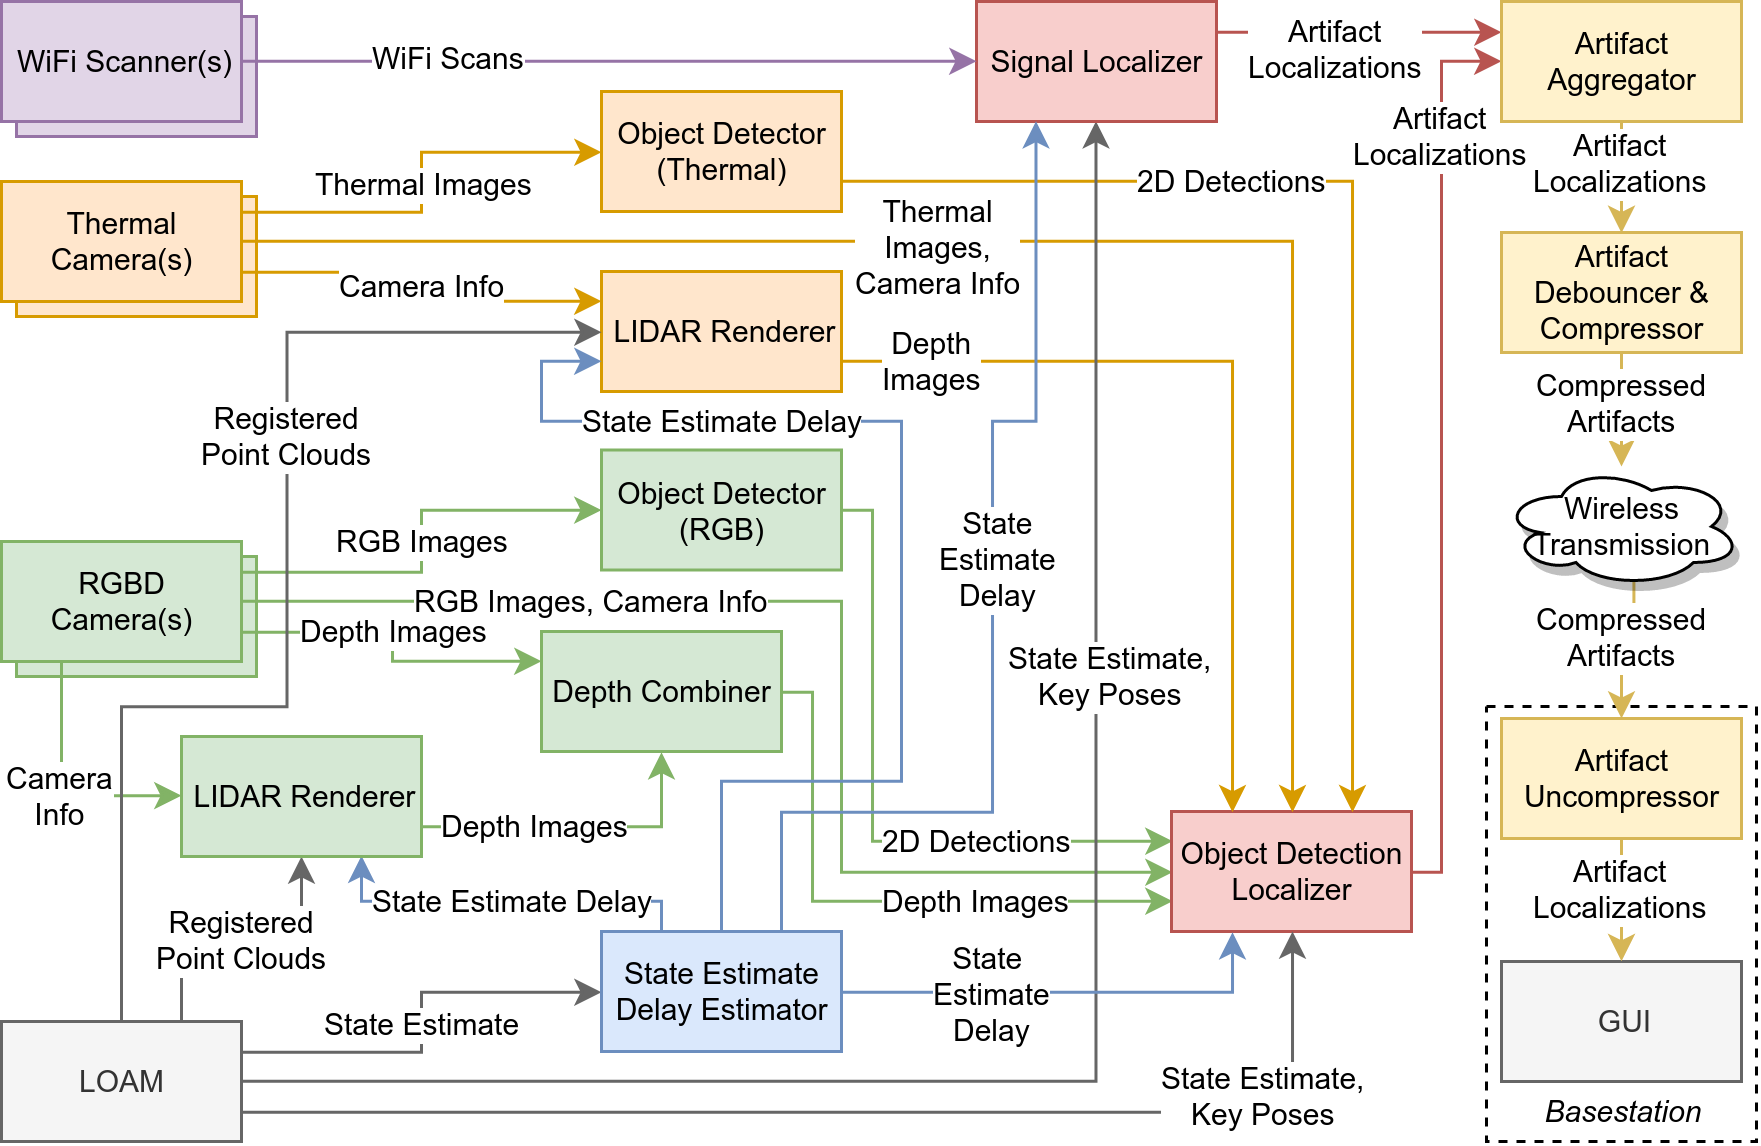
\includegraphics[width=\textwidth]{software_overview.png}
	\caption{Artifact detection and localization software diagram}
	\label{software_overview}
\end{figure}

% TODO(vasua): A better figure for what is inside an artifact localization?
The pipeline consists of 2 major modules - the Signal Localizer and the Object Detection Localizer. Each module takes in various sensor data and produces artifact localizations, which are 3D coordinates in the robot's map frame that are believed to correspond to a desired artifact. These artifact localizations may contain additional evidence to be displayed to the human supervisor, such as images or point clouds of the artifact and surrounding environment. Artifact localizations from both modules are combined inside the Artifact Aggregator and then transmitted to the base station to be displayed on the GUI. The human supervisor inspects artifacts displayed on the GUI and reports valid ones to DARPA.

\section{LOAM Overview}

One of the assumptions made during the initial design phases of the software pipeline was that LOAM would be the state estimation system used on all of our payloads. This simplified the development of the artifact detection and localization pipeline as we only needed to develop and test against a single state estimation system. The relevant interface details of LOAM (in the form of ROS frames and topics) are given below:

\begin{description}
	\item[/sensor] This is the robot's local frame, and is coincident with the Velodyne LIDAR's frame.
	\item[/sensor\_init] The fixed frame used as the base for LOAM's odometry.
	\item[/map] The world frame, which is initially coincident with sensor\_init but can change after loop closures.
	\item[/key\_pose\_to\_map] LOAM creates a series of key poses as the robot traverses the environment. These key poses are generated approximately every 2 meters of the robot's path. Each key pose is given a unique ID, starting from 0. The key pose is published relative to the /map frame.
	\item[/key\_pose\_path] When LOAM detects a loop closure, it corrects the key poses and publishes a new list of key pose IDs and poses.
	\item[/velodyne\_cloud\_registered] The laser scan from the Velodyne LIDAR is aligned to previous scans and published on this topic at 5 Hz. Contrary to key poses, registered scans are published on this topic even when the robot is stationary. The scans are registered in the /sensor\_init frame and accumulate drift over time, but are locally smooth.
	\item[/integrated\_to\_map] The 6DOF pose of the /sensor frame is published on this topic at 200 Hz. The pose is corrected by loop closures and thus does not accumulate significant drift, but may be discontinuous locally.
\end{description}

\section{Object Detector (RGB)}

TODO

\section{Object Detector (Thermal)}

TODO

\section{LIDAR Renderer}

The LIDAR renderer uses camera information (intrinsics and extrinsics) to render depth images. The depth information comes from the registered point clouds from LOAM. For RGB images, the LIDAR renderer provides an alternative source for depth information as depth images are already produced by the RealSense cameras. However, the LIDAR renderer serves as the only source of depth information for the thermal cameras, as they do not otherwise have associated depth information.

\subsection{Implementation}

Two implementations of the LIDAR renderer were created - a reference implementation which ran on CPU, and an optimized one which ran on a GPU using CUDA. The optimized implementation is used on both Mk. 0 and Mk. 1 and runs on the Xavier, where it renders depth images for either 5 or 6 image streams (4x RGB and 1 or 2x thermal). The reference implementation was used to validate the GPU implementation for correctness. The reference implementation also runs on the NUC on the drone payload as it does not have a GPU that supports CUDA. The slower performance of the reference implementation is acceptable as renders only need to be produced for a single RGB stream. Both implementations share the same overall algorithm, comprising two separate methods:

\begin{description}
	\item[Cloud aggregation] The renderer aggregates the registered point clouds from LOAM. A rolling buffer of these clouds is maintained, whose size is proportional to the time it takes to render an image. 10 clouds are stored in the reference implementation, and 30 clouds are stored in the GPU implementation. The clouds are already transformed into a common frame and form a locally smooth point cloud. Global drift is present, but can be ignored since the rendered depth images only see a small local portion of the map.
	\item[Rendering] For each rendered image, the renderer computes the position of the camera in the same frame as the aggregated point clouds. The renderer then uses the camera intrinsics to construct a pinhole camera model and projects each point through it to obtain a location in image coordinates. This coordinate, as well as pixels around this coordinate (based on a configurable inflation parameter) are updated based on the distance to the point, keeping the closer point. The projected coordinates are inflated (as shown in Figure \ref{lidar_inflate}) to provide a denser output image to ensure that depth values are not lost in any potential future downsampling.
\end{description}

\begin{figure}
	\centering
	\begin{subfigure}{0.3\textwidth}
		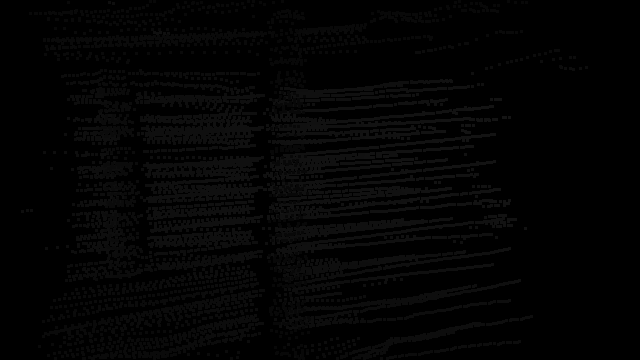
\includegraphics[width=\textwidth]{inflate_1.png}
		\caption{1 pixel inflation}
		\label{inflate_1}
	\end{subfigure}		
	\hfill
	\begin{subfigure}{0.3\textwidth}
		
\includegraphics[width=\textwidth]{inflate_4.png}
		\caption{4 pixel inflation}
		\label{inflate_4}		
	\end{subfigure}
	\hfill
	\begin{subfigure}{0.3\textwidth}
		
\includegraphics[width=\textwidth]{inflate_8.png}
		\caption{8 pixel inflation}
		\label{inflate_8}
	\end{subfigure}
	\caption[LIDAR renderer inflation values comparison]{Rendered images of the same scene with different inflation values. An inflation value of 4 was used for all payloads.}
	\label{lidar_inflate}
\end{figure}

\subsection{Results}

A selection of outputs from the LIDAR renderer is given in Figure \ref{lidar_renderer_images}, along with the depth image output from the RealSense camera and the associated RGB image for reference. In the first row, with Mk. 1's camera looking down a long tunnel, the rendered image is significantly sharper and more consistent than that of the RealSense. In the second row, with the left camera looking at a nearby wall, both depth images are similar. In the final row, with a scene from Mk. 1's back camera (which is tilted upwards), the RealSense depth image has significantly fewer holes than the LIDAR's due to the LIDAR's narrow vertical field of view. 

These results show that the output from the LIDAR renderer is either on par with, or better than that from the RealSense cameras, assuming the camera's full field of view is captured by the LIDAR. By fusing both depth images in the Depth Combiner, we can obtain better depth images than either source provides individually.

\begin{figure}
	\centering
	\begin{subfigure}{0.3\textwidth}
		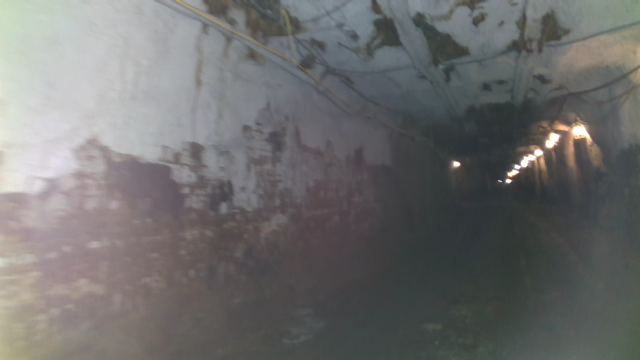
\includegraphics[width=\textwidth]{rs_front_example_2019-10-16-00-51-04_color.png}
		\caption{Mk. 1 Front Color}
		\label{lidar_front_color}
	\end{subfigure}		
	\hfill
	\begin{subfigure}{0.3\textwidth}
		
\includegraphics[width=\textwidth]{rs_front_example_2019-10-16-00-51-04_ref.png}
		\caption{Mk. 1 Front Depth}
		\label{lidar_front_ref}		
	\end{subfigure}
	\hfill
	\begin{subfigure}{0.3\textwidth}
		
\includegraphics[width=\textwidth]{rs_front_example_2019-10-16-00-51-04_render.png}
		\caption{Mk. 1 Front Rendered}
		\label{lidar_front_render}
	\end{subfigure}
	\\
	\begin{subfigure}{0.3\textwidth}
		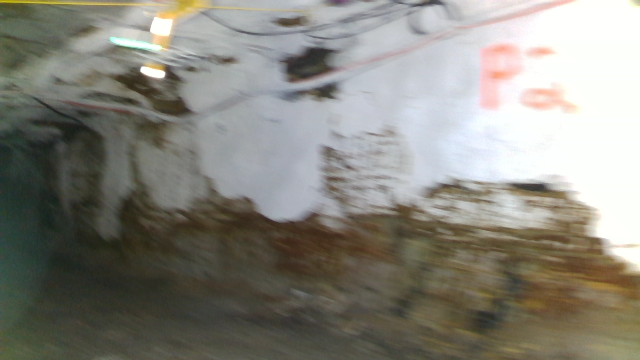
\includegraphics[width=\textwidth]{rs_left_example_2019-10-16-00-51-02_color.png}
		\caption{Mk. 1 Left Color}
		\label{lidar_left_color}
	\end{subfigure}		
	\hfill
	\begin{subfigure}{0.3\textwidth}
		
\includegraphics[width=\textwidth]{rs_left_example_2019-10-16-00-51-02_ref.png}
		\caption{Mk. 1 Left Depth}
		\label{lidar_left_ref}		
	\end{subfigure}
	\hfill
	\begin{subfigure}{0.3\textwidth}
		
\includegraphics[width=\textwidth]{rs_left_example_2019-10-16-00-51-02_render.png}
		\caption{Mk. 1 Left Rendered}
		\label{lidar_left_render}
	\end{subfigure}
	\\
	\begin{subfigure}{0.3\textwidth}
		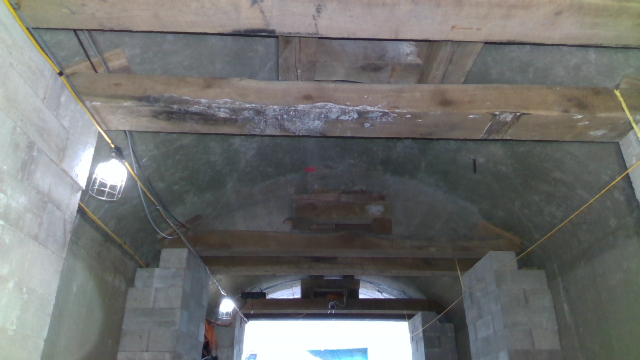
\includegraphics[width=\textwidth]{rs_back_example_2019-10-16-00-33-41_color.png}
		\caption{Mk. 1 Back Color}
		\label{lidar_back_color}
	\end{subfigure}		
	\hfill
	\begin{subfigure}{0.3\textwidth}
		
\includegraphics[width=\textwidth]{rs_back_example_2019-10-16-00-33-41_ref.png}
		\caption{Mk. 1 Back Depth}
		\label{lidar_back_ref}		
	\end{subfigure}
	\hfill
	\begin{subfigure}{0.3\textwidth}
		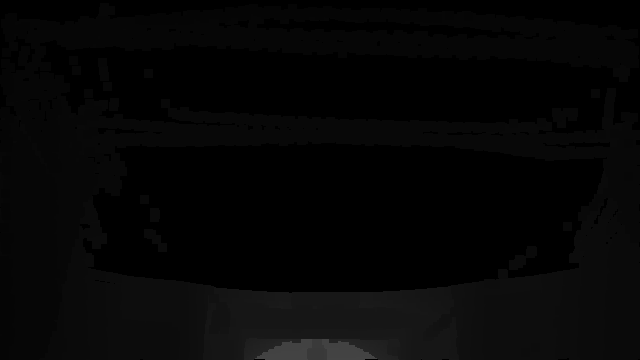
\includegraphics[width=\textwidth]{rs_back_example_2019-10-16-00-33-41_render.png}
		\caption{Mk. 1 Back Rendered}
		\label{lidar_back_render}
	\end{subfigure}		
	\caption[LIDAR renderer depth image comparison]{Comparison of depth images generated by the LIDAR renderer to depth images from the RealSense cameras. Color images, captured simultaneously by the RealSense cameras, are provided for reference.}
	\label{lidar_renderer_images}
\end{figure}

\section{Depth Combiner}

The depth combiner fuses depth images from the RealSense depth camera and LIDAR renderer into a single depth image to be used in the object detection localizer. The two image streams are aligned, and can thus be fused per-pixel. The following equation was used (shown as C++ code):

\begin{lstlisting}[language=c++]
fused = (realsense > threshold || realsense == 0) ? lidar : realsense;
\end{lstlisting}

This fusion keeps lidar data whenever the reported RealSense data is either not present (\lstinline[language=c++]{realsense = 0}) or exceeds some threshold (\lstinline[language=c++]{realsense > threshold}). The threshold empirically selected to be 2.5m, which is the approximate distance after which we observed significant variance in reported depth values between frames. This fusion allows us to use the high density RealSense depth information whenever it is available and sufficiently accurate (under the 2.5m threshold), and utilize the sparser LIDAR information otherwise. An example output is given in Figure \ref{combined_depth}.

\begin{figure}
	\centering
	\begin{subfigure}{0.3\textwidth}
		
\includegraphics[width=\textwidth]{rs_back_example_2019-10-16-00-33-41_ref.png}
		\caption{Mk. 1 Back Depth}
		\label{combined_depth_realsense}		
	\end{subfigure}
	\hfill
	\begin{subfigure}{0.3\textwidth}
		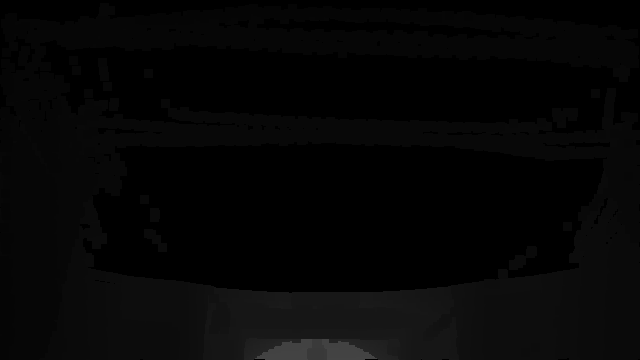
\includegraphics[width=\textwidth]{rs_back_example_2019-10-16-00-33-41_render.png}
		\caption{Mk. 1 Back Rendered}
		\label{combined_depth_lidar}
	\end{subfigure}	
	\hfill
	\begin{subfigure}{0.3\textwidth}
		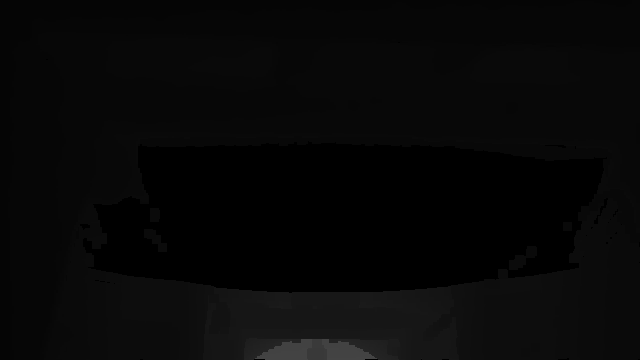
\includegraphics[width=\textwidth]{combined_depth.png}
		\caption{Mk. 1 Back Combined}
		\label{combined_depth_output}
	\end{subfigure}		
	\caption[Depth combiner sample output]{Example of the output from the depth combiner, using the same scene as in \ref{lidar_back_color}.}
	\label{combined_depth}
\end{figure}


\section{Object Detection Localizer}

TODO

\section{WiFi Scanner}

TODO

\section{Signal Localizer}

TODO

\section{State Estimate Delay Estimator}

TODO

\section{Artifact Aggregator}

TODO

\section{Artifact Debouncer \& Compressor}

TODO

\section{Artifact Uncompressor}

TODO

\section{GUI}
\chapter{Experiments and Results}

During the Tunnel Circuit, we deployed our complete system, comprising 2 ground robots (R1, R2) and a drone (D1) a total of 4 times over 4 days. For the 1st and 4th days, we operated in the Experimental mine, while on the 2nd and 3rd days we operated in the Safety Research Mine. The second run for each mine had a different set of artifacts and locations than the first. The final scores for each deployment, as recorded by DARPA, are shown in Table \ref{final_scores}. Each configuration had 20 artifacts deployed.

\begin{table}
	\centering
	\begin{adjustbox}{max width=.95\textwidth}
		\csvreader[
		respect underscore=true,
		tabular=|l|c|c|,
		late after line=\\\hline,
		table head=\hline \textbf{Course Name} & \textbf{Artifact Configuration} & \textbf{Official Score}\\\hline,
		]{final_scores.csv}{}{\csvlinetotablerow}
	\end{adjustbox}
	\caption{Official scores from Tunnel Circuit}
	\label{final_scores}
\end{table}

\section{Experimental Setup}

After the Tunnel Circuit, a number of experiments were performed to determine the utility and performance of each part of the system. All experiments were performed by playing back data recorded on R2  (which carried the Mk. 1 payload) on day 2, in the Safety Research mine with artifact configuration A. Ground truth artifact locations for this configuration were obtained by transforming the ground truth provided by DARPA after the competition into R2's /map frame using the calibration determined at competition. The calibration was not updated between experiments. This transformation allowed all experiments to take place in R2's /map frame, rather than requiring a transformation of artifact coordinates during experiments. A map of the Safety Research mine, artifact locations, as well as the areas traversed by R2 on day 2 is given in Figure \ref{tunnel_circuit_day_2}.

\begin{figure}	
	\centering
	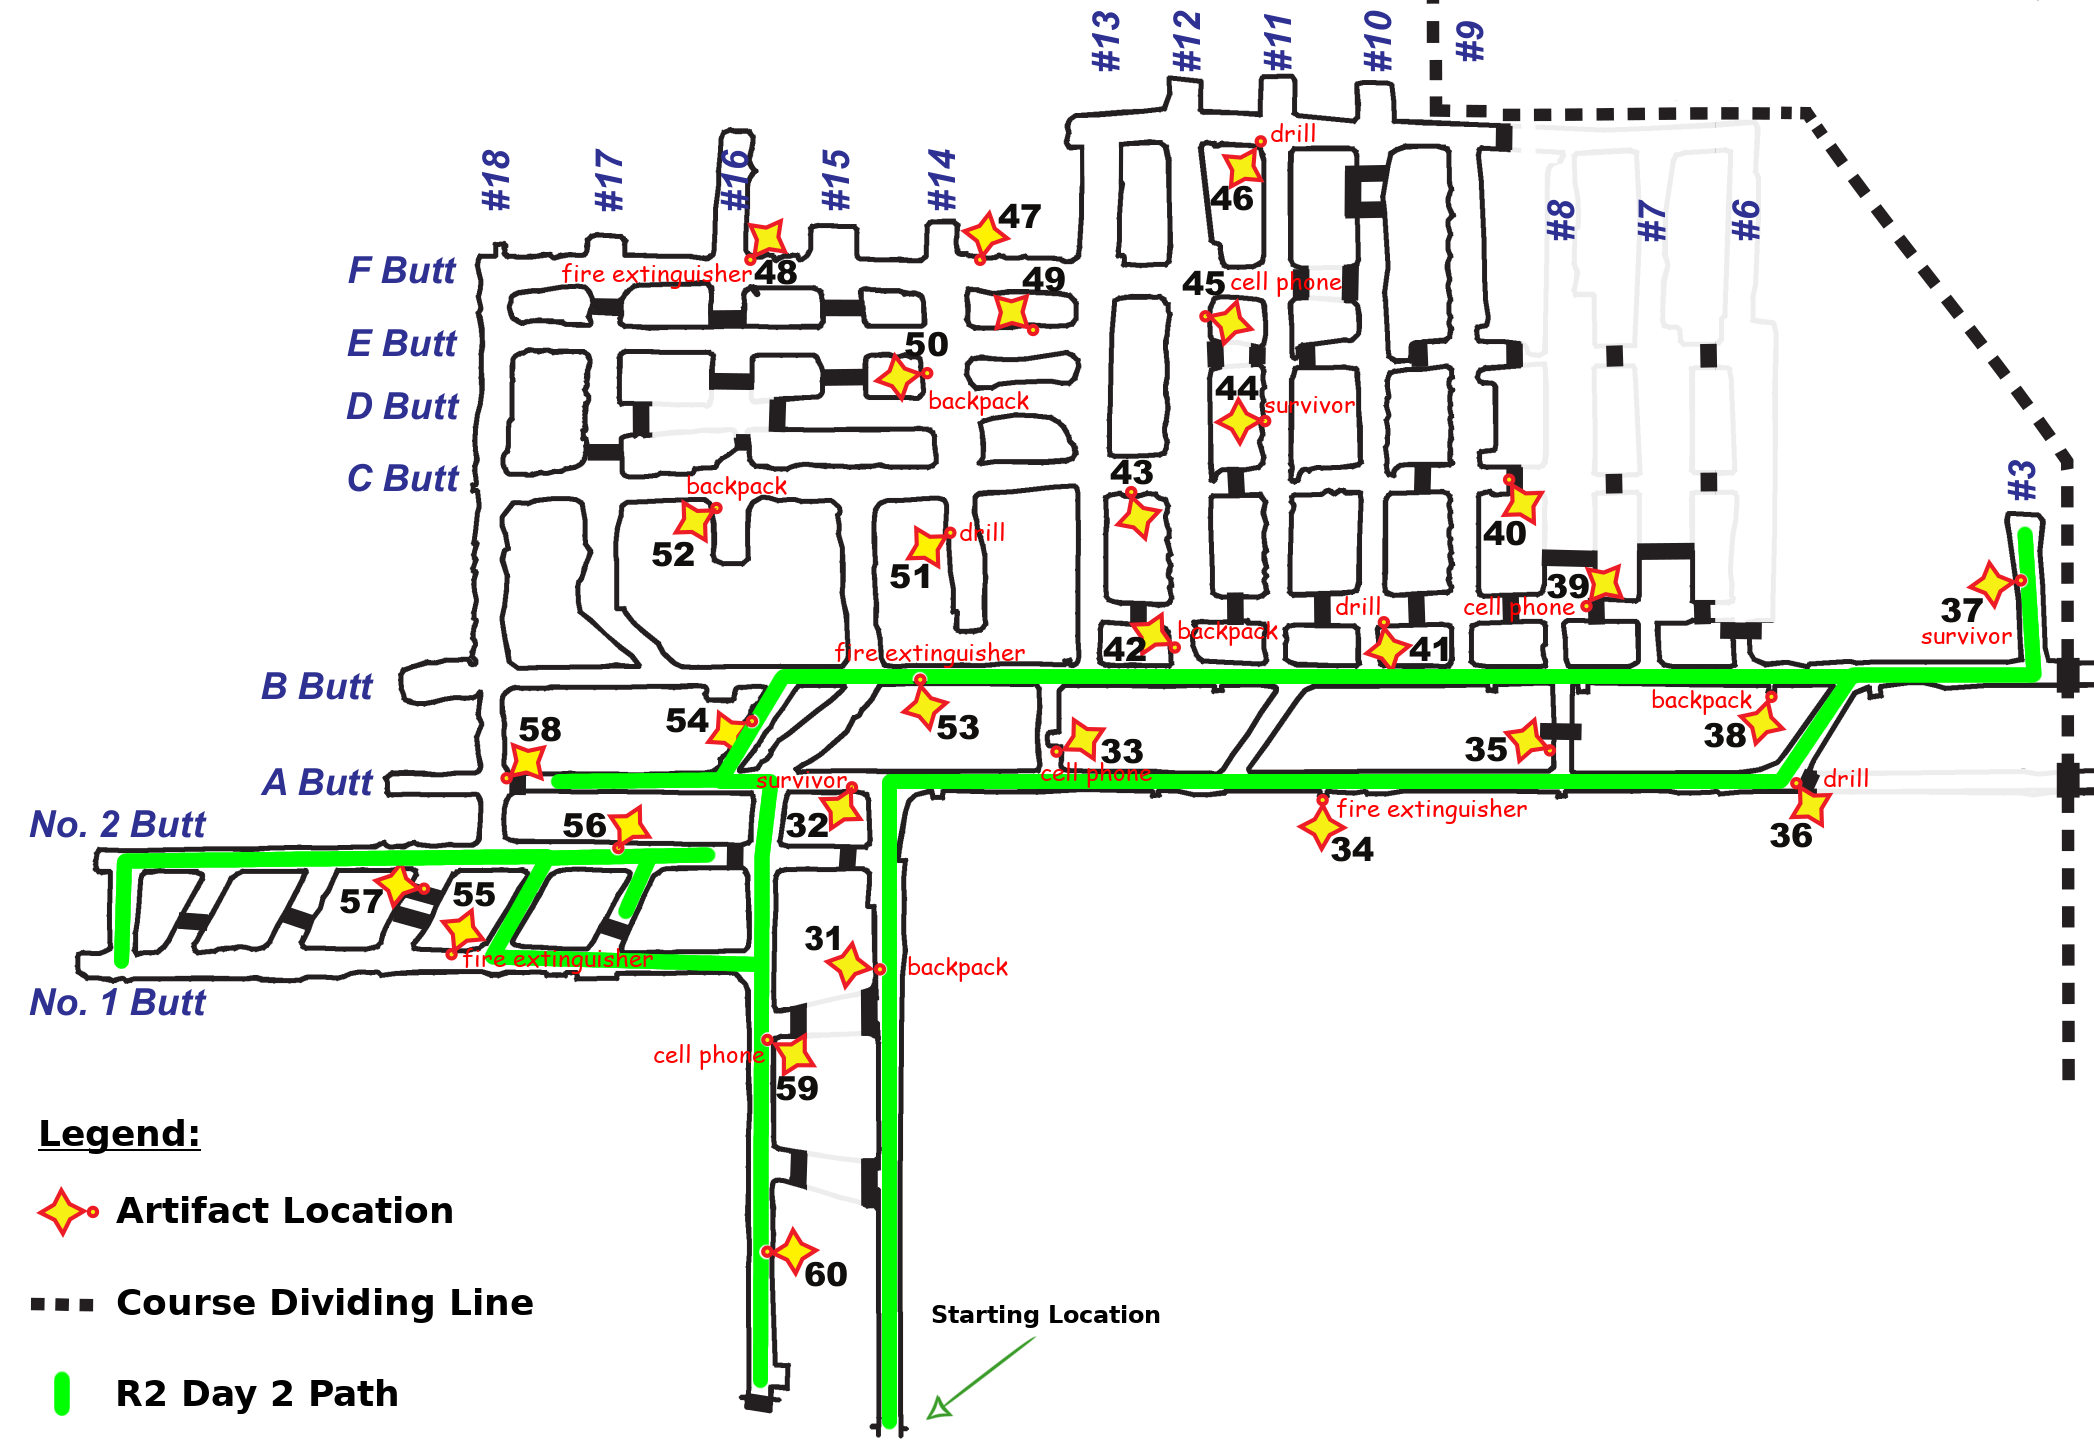
\includegraphics[width=\textwidth]{Tunnel_Artifact_Map_day_2.png}
	\caption[Tunnel Circuit day 2 artifact locations]{Ground truth locations for artifacts in the Safety Research mine during day 2 of the Tunnel Circuit. Numbers with text represent locations where artifacts were actually present. Locations without text did not contain artifacts. The cell phone at location 33 was not broadcasting an access point during this day due to a confirmed error by DARPA. The robot started at the right tunnel in the center of the figure and turned around after reaching No. 1 Butt after approximately 20 minutes.}
	\label{tunnel_circuit_day_2}
\end{figure}

During each experiment, the system reported artifacts directly to a scoring server, rather than reporting them to the base station for human verification. While this setup is slightly different than that used during competitions, it enables more consistent and repeatable experiments and allows multiple experiments to be run in parallel. The scoring server aggregates all artifacts reported by the system similarly to other nodes, and scores the entire list of artifacts whenever an update is received. Artifacts are scored by matching valid artifacts to ground truth artifacts, ensuring that the reported artifact is within 5m Euclidean distance of the ground truth artifact and shares the same class. Precision is determined according to Equation \ref{precision_equation}. The results are appended to a file on disk, allowing the system's performance over time to be analyzed.

\begin{equation} \label{precision_equation}
precision = \frac{\#\ correct\ artifacts}{\#\ valid\ artifacts}
\end{equation}

Streaming results directly to the server also removes the effect of communication network, assuming instead that the robot is always able to communicate with the base station. An analysis of the actual bandwidth usage under different configurations of the artifact compressor for the R2 day 2 dataset is given in Figure \ref{bandwidth_usage}. 

The results of each experiment are compared to the results of the configuration used during the Tunnel Circuit, described in Figure \ref{software_overview}. Values in plots indicating the number of artifacts detected have been slightly altered by adding an offset of between -3\% and 3\% to all values to improve legibility. Values in all other plots have not been altered.

\section{Single Sensor Usage}

Our core hypothesis for this work is that the use of multiple sensors and sensing modalities is necessary and advantageous in detecting and localizing artifacts. To test this hypothesis, as well as to understand the utility of each individual sensor, the artifact detection and localization pipeline was run with only a single sensor active at once. Each of the 4 RGB cameras and 2 thermal cameras were run separately, while both radios feeding the signal localizer were run simultaneously. The results are shown alongside the full system with all sensors active simultaneously in Figure \ref{sensors_vs_full}.

\begin{figure}	
	\centering
	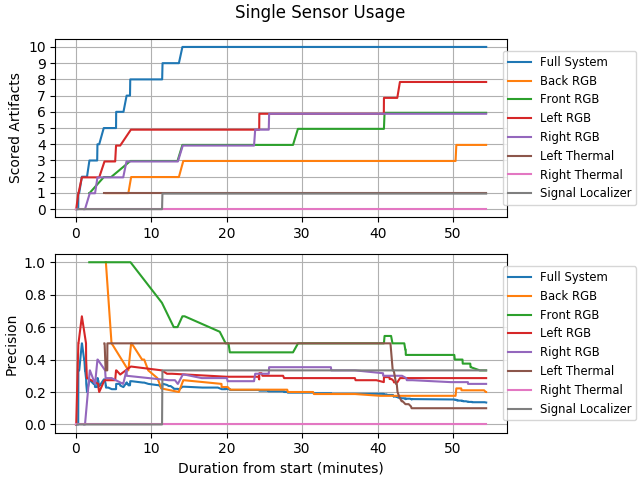
\includegraphics[width=\textwidth]{eval_graphs/sensors_vs_full.png}
	\caption[Single sensor artifact localization]{The plot shows the results from configurations in which only a single sensor was active. Both radios were used simultaneously for the signal localizer.}
	\label{sensors_vs_full}
\end{figure}

When combining all of the sensors, the robot was able to score all 10 artifacts in its path by approximately 15 minutes. No single sensor was able to achieve the same score, even at the end of the competition run. A total of 9 artifacts could have been detected by each RGB camera, which is all artifacts except the cell phone at location 59 in Figure \ref{tunnel_circuit_day_2}. Each RGB camera scored most, but not all, of the artifacts in the robot's path, and required the robot to turn around and back to the entrance of the tunnel, which happened at approximately 20 minutes into the run. Using the full system, the robot would instead be able to keep exploring and continue to report information for situational awareness. 

Two survivor artifacts were present along the robot's path which could have been detected by the thermal cameras. When using only the left thermal camera, only 1 survivor artifact was scored. None were scored by the right thermal camera. This may be attributed to a lower quality thermal object detector as a result of fewer training examples, or the low framerate of thermal detection (5 Hz) preventing sufficient confidence from accumulating to consider a detected object an artifact.

The signal localizer is the only module capable of localizing cell phones, and was able to score the single cell phone artifact (59) acting as a WiFi access point along its path (59). The other two broadcasting cell phone artifacts (39, 45) were detected by the WiFi scanner but could not be localized sufficiently accurately by the signal localizer since the robot did not traverse the areas near the artifacts.

While each individual sensor had a lower overall score than the complete system, all sensors except the thermal cameras resulted in a higher precision than the overall system. This may be due to the fact that all configurations used the same confidence thresholds for determining when to publish an Artifact Localization. When only a single sensor is used, more false positive detections are required per sensor to create a false positive Artifact Localization than when all sensors are fused together. The higher false positive rate for the full system is acceptable based on the team's concept of operations, but this experiment may indicate an opportunity to lower the false positive rate by dynamically adapting confidence thresholds based on the number of sensors being fused.

\section{RealSense Depth Only}

During the development process, we discovered that the RealSense camera's depth accuracy drops significantly after approximately 2.5m. As a result, depth information from the RealSense is discarded after 2.5m and replaced with depth information from the LIDAR in the full system. This experiment quantifies the utility of the fusion of LIDAR data by examining the system performance with only a single RealSense activated and limited to using only RealSense depth information under 2.5m. The results are shown in Figure \ref{rs_depth_only}.

\begin{figure}	
	\centering
		\begin{subfigure}{0.48\textwidth}
			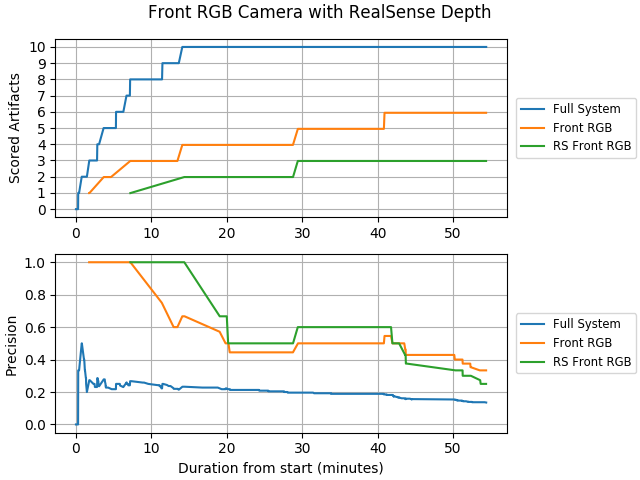
\includegraphics[width=\textwidth]{eval_graphs/rs_depth_front.png}
			\label{rs_depth_front}
		\end{subfigure}
		\hfill
		\begin{subfigure}{0.48\textwidth}
			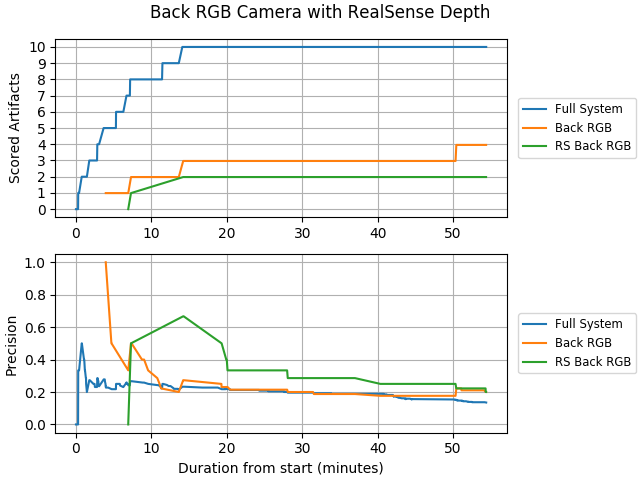
\includegraphics[width=\textwidth]{eval_graphs/rs_depth_back.png}
			\label{rs_depth_back}
		\end{subfigure}
		\\
		\begin{subfigure}{0.48\textwidth}
			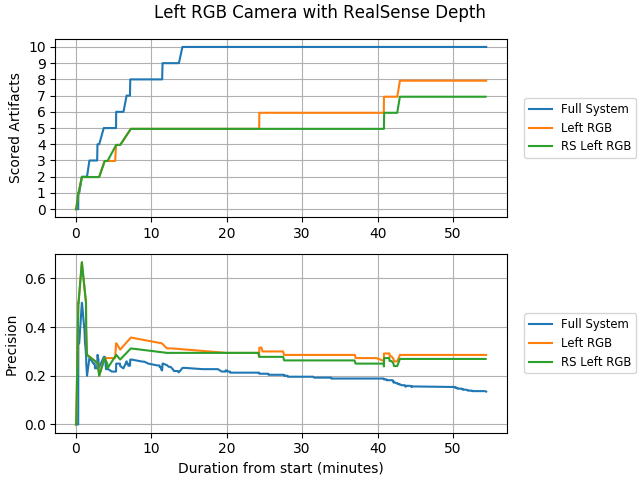
\includegraphics[width=\textwidth]{eval_graphs/rs_depth_left.png}
			\label{rs_depth_left}
		\end{subfigure}
		\hfill
		\begin{subfigure}{0.48\textwidth}
			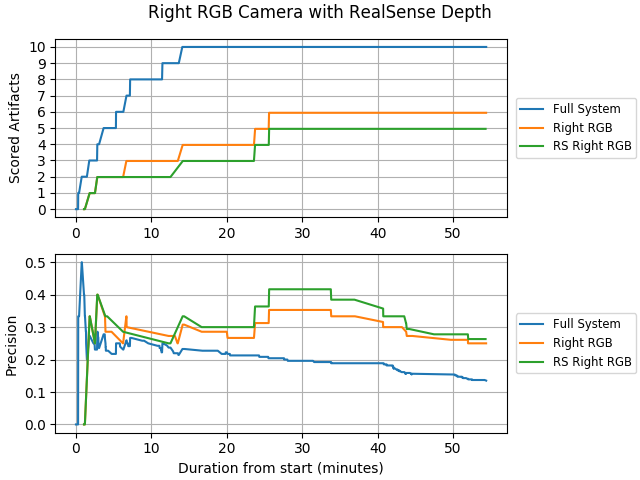
\includegraphics[width=\textwidth]{eval_graphs/rs_depth_right.png}
			\label{rs_depth_right}
		\end{subfigure}
	\caption[Single RGB sensor scores using only RealSense depth]{Only the RealSense depth information was used to localize artifacts in this test, resulting in an effective detection range of 2.5m for the RGB cameras.}
	\label{rs_depth_only}
\end{figure}

The front and back cameras have the largest decrease in accuracy when utilizing only RealSense depth information, with each scoring only half of the artifacts scored when fusing LIDAR information. This is likely due to the topology of the environment itself. The Tunnel Circuit environment consists of many narrow corridors. When the robot drives by artifacts and they are detected by the left and right RGB cameras, the artifact is typically very close to the robot. In contrast, the front and back cameras are typically looking down the long corridors and thus artifacts are often beyond the 2.5m threshold. The precision of each of the RGB cameras with both types of depth information is comparable and significantly higher than that of the full system.

\chapter{Conclusions and Future Work}

This work comprises the development of three separate payloads and a scalable and flexible software system running on each payload capable of providing rapid situational awareness in the form of Artifact Localizations for the DARPA Subterranean Challenge. Each of the three payloads (drone, Mk. 0, and Mk. 1) contains a variety of sensors and sensing modalities which are fused to provide a single, globally consistent list of artifacts to a human operator at the base station in a robust and timely manner. This simulates information being reported first responders and emergency personnel during a disaster scenario, where rapid and accurate information about the environment is critical to saving lives and mitigating damage.

The complete system was tested during a number of field experiments, culminating in a series of deployments during the Tunnel Circuit of the DARPA Subterranean Challenge. We reported 25 out of 40 artifacts correctly between the two portals (Safety Research, Experimental), and won first place out of the 11 teams at the event. We also won an award for reporting the most accurate artifact, a backpack artifact reported during the second deployment in the Safety Research portal, with an error of 0.18m. Using the data collected at the Tunnel Circuit, we demonstrate the advantage and necessity of the fusion of multiple sensors and sensing modalities, which results in more artifacts being found, and being found more quickly, than is possible with any single sensor.

Many avenues for improvement of the system exist. Hardware synchronization for timestamps between all sensors in the payloads would result in a more consistent registration of sensor data to state estimates. Explicit modeling of localization points on each artifact could help remove between 10 cm and 1 m of error for each artifact report. An improved dataset and object detection model would reduce the number of false positives detected, increasing precision. Adding a form of segmentation to object detection would remove points in the environment from the calculation of artifact locations. An environment-aware cell phone trilateration strategy would enable accurate cell phone localization in a multitude of environments and would remove the current requirement of proximity. The microphone array and LIDAR could be used to detect additional artifact categories, or provide additional evidence for existing ones. These changes, and many others, would improve the Artifact Localizations reported by the system and thus the quality of the situational awareness provided to future base station operators, including first responders and emergency personnel.

%\appendix
%\include{appendix}

\backmatter

%\renewcommand{\baselinestretch}{1.0}\normalsize

% By default \bibsection is \chapter*, but we really want this to show
% up in the table of contents and pdf bookmarks.
\renewcommand{\bibsection}{\chapter{\bibname}}
%\renewcommand{\bibpreamble}{This text goes between the ``Bibliography''
%  header and the actual list of references}
\bibliographystyle{plainnat}
\bibliography{references} %your bib file

\end{document}
